\chapter{Union-Find Balanced Bloom decoder}\label{ch:ufbb}

\tikzstyle{node}=[circle, draw=black, fill=white, minimum size=25pt, line width=1, inner sep= 5pt]
\tikzstyle{nodel}=[circle, draw=black, fill=white, minimum size=15pt, line width=1, inner sep= 0pt]
\tikzstyle{node1}=[circle, draw=black, fill=white, minimum size=15pt, line width=1, inner sep= 2pt]
\tikzstyle{node2}=[circle, draw=black, fill=white, minimum size=8pt, line width=1, inner sep= 0pt, fill=white!70!black]
\tikzstyle{l1}=[line width=1]
\tikzfading[name=fade right, left color=transparent!0, right color=transparent!100]

% Recall that in the Union-Find decoder, each cluster represented by a set of vertices $C_i = |\{v_1, v_2, ...\}$ stored as a disjoint-set tree of the Union-Find data structure. To find the parent cluster of any given vertex, we follow subsequent parent pointers to the root vertex of the tree, which is the representative element of the cluster. Merges between clusters is done by simply pointing the root of one tree to another. By implementing additional rules \emph{path compression} and either \emph{union by weight} or \emph{union by rank}, the heights of the trees are dynamically kept low, such that the overall complexity of the algorithm for a system of $n$ qubits is $n\alpha(n)$, where $\alpha(n)\leq 4$ for all physical values of $n$. 

In this chapter we describe a modification of the UF-decoder, dubbed the \emph{Union-Find Balanced-Bloom} decoder, that increases the code threshold of the UF-decoder by improving its heuristic for minimum-weight matchings. We show that the modified decoder retains a relatively low time-complexity. 

Within the vanilla UF-decoder, not all odd-parity clusters are grown at the same time. Larger clusters relatively add more "incorrect edges" to themselves than compared to a smaller cluster (lemma \ref{lem:incorrectedges}). The UF decoder therefore applies \emph{weighted growth} of clusters, where the order of cluster growth is sorted based on the cluster sizes. We have shown a linear time implementation utilizing \emph{bucket sort} in Section \ref{sec:bucketwg}. With the addition of weighted growth, the error threshold of the UF decoder is reported to increase from $9.2\%$ to $9.9\%$ for a 2D toric lattice \cite{delfosse2017almost}, whereas we measured an increase from $9.716\%$ to $9.984\%$ in our implementation of the decoder (Section \ref{sec:ufperformance}). Furthermore, we showed that by always maintaining a dynamic forest where all clusters are connected acyclic graphs (Section \ref{sec:dynamicforest}), a slight increase in the code threshold and reduced running time can be obtained. 

From the simulated results of several of our implementations of the Union-Find decoder (Section \ref{sec:ufimplementations}), we grew the intuition that a decreased weight is to some extend a heuristic for an increased code threshold (formalized in Proposition \ref{prop:mw2}). In fact, the instruction of the Union-Find decoder mostly tries to obtain a low weight matching; by growing the odd-parity clusters on their boundaries a single layer at the time, unions between odd-parity clusters mostly occur on nearest neighbors. The discrete coordinates of the lattice limits the number of growth iterations to a constant proportional to the lattice. But also due to this discreteness, there may be many unions within each growth iteration, and nearest-neighbor unions between clusters may not result in a minimum-weight matching between syndromes. Especially as the clusters increase in size, also does their boundaries, and a increasingly larger amount of "incorrect edges" are added to the cluster. Weighted grow reduces the number of large-cluster growths, but does not decrease the number of "incorrect edges" if a large cluster is grown. This leaves us with the question: Should all boundary edges of a cluster be grown simultaneously?

% A large cluster is generally the result of multiple rounds of growth of a smaller cluster. Each iteration of cluster growth buries the syndromes within that cluster with a layer of edges, of which only a small portion will be part of the matching, where each layer adds to the matching weight. With weighted growth, smaller clusters are grown first, such that this effect is less dominant. But the UF decoder is unsurprisingly less successful at minimum-weight than the MWPM decoder, which does this perfectly. The MWPM decoder considers all possible matchings by constructing a fully connected graph where the edges have the distance between syndrome as weights. The UF decoder does not look at the lattice in such a global way, but performs locally on each cluster. This should yield the same result conceptually, but in reality it does not due to a major weakness; In each round of growth, all boundary edges are grown simultaneously. The potential union of two clusters is reserved to one edge but may occur on many, is only handled after each round, where the order of the merging edges determines which edge is selected as the bridge.
We suspect that the error threshold of the Union-Find decoder can be increased by improving the heuristic for minimum-weight matchings. In this chapter, we accomplish this by sorting the growth of specific subsets ofa cluster according to a parameter that we dub the \emph{potential matching weight}, explained in \ref{sec:PMW}. We introduce a new data structure that we call the \emph{node set} of a cluster in \ref{sec:nodeset}. Within this node set, we compute the node \emph{parity} and \emph{delay} in \ref{sec:nodedelay} and \ref{sec:bbstate}, which sets the order of boundary edge growth. In \ref{sec:growingcluster} through \ref{sec:multiplejoint}, we cover the rules for growth and join operations for the node sets, which are more complex than those of the UF algorithm. The modified decoder, the Union-Find Balanced-Bloom decoder, still has a relatively low worst-case quasilinaer time complexity, which is approximated in \ref{sec:ufbbcomplexity}. 

\section{A potential matching weight}\label{sec:PMW}

The Minimum-Weight Perfect Matching decoder finds the minimum-weight subset of edges by constructing a fully connected graph between all vertices (Section \ref{sec:MWPMdecoder}). By computing on the entire lattice, we denote such decoder as a \emph{global} decoder. The Union-Find decoder is a \emph{local} decoder, as each cluster is grown individually, oblivious about its surrounding neighbors until it merges into them. We introduce in this section the concept of a \emph{potential matching weight} of an odd-parity cluster, and we show that its value is not constant across the vertices of a cluster.

\begin{definition}\label{def:pmw}
  Consider an odd-parity cluster $c_i$ containing a vertex $v$. The Potential Matching Weight (PMW) of the vertex $v$ is the matching weight in the subset of edges of an odd-parity cluster $c_i$ in a hypothetical union with another cluster $c_j$ in the next growth iteration, where the merging boundary edge is supported by $v$. 
  \begin{equation}
    PMW(v) = \abs{\m{C} \cap \m{E}_{i}} \text{ if } c_i, c_j \text{ merged by } \codefunc{Union}(v,u) | v \in \m{V}_{i}, u \in \m{V}_{j}, 
  \end{equation}
\end{definition}

Recall from Definition \ref{def:cluster} that a cluster with index $i$ is defined as a object $c_i$ with an edge set $\m{E}_i$ and vertex set $\m{V}_i$. 


Let us first consider an example. Cluster $C_e$ is defined by vertex set $\vset_e = \{v_1, v_2, v_3\}$ (Figure \ref{fig:PMW}). The vertices lie on a horizontal line, distance 1 from each other, where each vertex has grown a single iteration of half-edges. Assume that each vertex in $\vset_e$ is a syndrome, it has odd parity and is selected for growth. As UF decoder performs on the cluster locally, it has no knowledge about the state of its surrounding vertices until the cluster grows and merges with them. 

Now let us investigate the weights of a matching if an additional vertex $v'$ is connected to the cluster.
If $v'$ is connected to $v_1$ or to $v_3$, then the resulting matchings have a total weight of 2: $(v',v_1)$ and $(v_2,v_3)$, or $(v',v_3)$ and $(v_1,v_2)$. However if $v'$ is connected to vertex $v_2$, then the total weight is 3: $(v', v_2)$ and $(v_1, v_3)$. This hypothetical weight after matching is the Potential Matching Weight (PMW) of a vertex.

From the above example, we can see that even for a minimal size odd cluster that is not a single vertex, the PMW is not equal for all vertices in the cluster. It would therefore not be "fair" to grow all boundary edges simultaneously. The growth of boundary edges connected to vertices with a high PMW should thus be delayed for some iterations, such that PMW's in the cluster reach the same value. However, if the PMW is to be calculated for every vertex with boundary edges in all clusters in every growth iteration, the time complexity of the algorithm would increase dramatically. Luckily, we can reduce these calculations to be performed on a set of \emph{nodes} in each cluster, which we clarify in the next section.

\begin{figure}
  \centering
  \vspace{1em}
   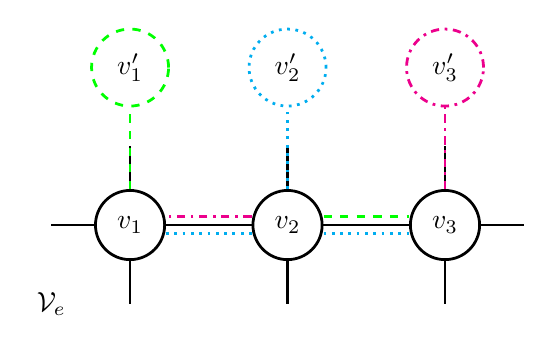
\begin{tikzpicture}
    \node at (-1, -1) {$\mathcal{V}_e$};
    \draw[l1] (0, 0) -- (4,0);
    \draw[l1] (-1,0) -- (5,0);
    \draw[l1] (0,1) -- (0,-1);
    \draw[l1] (2,1) -- (2,-1);
    \draw[l1] (4,1) -- (4,-1);
    \node[node] at (0,0) (1) {$v_1$};
    \node[node, draw=green, dashed] at (0,2) (2) {$v_1'$};
    \node[node] at (2,0) (3){$v_2$};
    \node[node, draw=cyan, dotted] at (2,2) (4) {$v_2'$};
    \node[node] at (4,0) (5) {$v_3$};
    \node[node, draw=magenta, dashdotted] at (4,2) (6) {$v_3'$};

    \draw[l1, dashed, green] (1) -- (2);
    \draw[l1, dashed, green, transform canvas={yshift=3pt}] (3) -- (5);
    \draw[l1, dotted, cyan] (3) -- (4);
    \draw[l1, dotted, cyan, transform canvas={yshift=-3pt}] (1) -- (3) -- (5);
    \draw[l1, dashdotted, magenta] (5) -- (6);
    \draw[l1, dashdotted, magenta, transform canvas={yshift=3pt}] (3) -- (1);

  \end{tikzpicture}
  \caption{Unbalanced matching weight in cluster vertex set $\mathcal{V}$. The matching edges (dashed) correspond to the position of $v'$. If $v'$ is connected to $v_1$ or $v_3$, the resulting matchings have a weight of 2. IF $v'$ is connected to $v_2$, the resulting matching has a weight of 3.}\label{fig:PMW}
\end{figure}

\section{Node set representation of cluster}\label{sec:nodeset}

To efficiently calculate the PMW's in a cluster, we introduce here an additional data structure, the \emph{node set} of a cluster. In the case of only Pauli errors, after syndrome identification, all identified clusters consist of a single vertex $v_i$ which are non-trivial syndromes $\sigma_i$. This set of clusters is equivalent to the syndrome set $\m{S}$. Within syndrome validation, these clusters are subjected to growth and merge events with other clusters. During growth, all vertices that are added to some cluster $C$ have a closest syndrome $\sigma$ within $C$ that is in the syndrome set $\m{S}$. The growth where vertices are added to a section of the cluster with a syndrome at the center can figuratively be compared with the \emph{bloom} of a flower, where all vertices in this section are \emph{seeded} in $\sigma$ and are called the flower of $\sigma$. 

Let us call these seeds the \emph{nodes} $n_i$ of the cluster. From our previous example, each vertex in $C_e$ is a syndrome in $\m{S}$, and is therefore a node. The node set is thus $\nset_e = \{n_1, n_2, n_3\} = \{\sigma_1, \sigma_2, \sigma_3\}$ where $\sigma_1 \equiv v_1$, $\sigma_2 \equiv v_2$ and $\sigma_3 \equiv v_3$. The number of vertices in $C_e$ increases in each round of growth by the bloom of the nodes in the cluster. However, the number of nodes remains the same at 3 nodes (Figure \ref{fig:nodesetpmw}). Moreover, as the bloom of a node adds vertices to the flower in all directions, all boundary vertices seeded in the same node are at equal distance to the syndrome at the center. Hence the PMW's for these boundary vertices are equal. The calculation of PMW's in the cluster thus does not require to traverse all the vertices, but just the nodes set of the cluster.

\begin{lemma}
  The calculation of PMW in the cluster can be limited to the nodes of a cluster, where all boundary vertices seeded in a node have the same PMW.
\end{lemma}

\begin{figure}
 \centering
 \begin{tikzpicture}
 
   \path[pattern=dots, pattern color=green] (0,3) arc (90:225:1) arc (45:-135:.4142) arc (45:315:1) arc (135:-45:.4142) arc (135:405:1) arc (225:135:.4142) arc (-45:45:1) arc (225:135:.4142) arc (-45:90:1) -- cycle;
   \path[pattern=grid , pattern color=cyan] (2,1) arc (90:450:1);
   \node[node, fill=white!70!green] at (0,0) (0) {$v_1$};
   \node[node, fill=white!70!cyan] at (2,0) (1) {$v_2$};
   \node[node, fill=white!70!black, path fading=fade right] at (4,0) (5) {$v_3$};
   \node[node] at (-2,0) (2) {$v_4$};
   \node[node] at (0,2) (3) {$v_5$};
   \node[node] at (0,-2) (4) {$v_6$};
   \draw[l1] (1) -- (0) -- (3);
   \draw[l1] (2) -- (0) -- (4);
   \draw[l1, dotted] (2, 1.5) -- (1) -- (2,-1.5);
   \draw[l1] (1) -- (5);
   

   \node at (-2, 2.5) {$\mathcal{V}_e$};
   \node at (7, 2.5) {$\mathcal{N}_e$};

   \node[node, pattern=dots, pattern color=green] at (7,0) (d) {$\sigma_1$};
   \node[node, pattern=grid , pattern color=cyan] at (9,0) (e) {$\sigma_2$};
   \node[node, fill=white!70!black, path fading=fade right] at (11,0) (f) {$\sigma_3$};
   \draw[l1] (d) -- (e) -- (f);
  \end{tikzpicture}
  \caption{A node set $\mathcal{N}$ vs. a vertex set $\mathcal{V}$, both representing the same cluster. Each shaded area covers the vertices of a different  node.}\label{fig:nodesetpmw}
\end{figure}

\subsection{Balanced Bloom}

The node set $\m{N} = \{n_1, n_2, .... n_{S_{\nset}}\}$ is stored as a tree, an connected and acyclic graph, where the edges $\epsilon$ between the nodes are the branches in our figurative flower bush. Each node-edge $\epsilon$ can have arbitrary length and consists of one or more vertex-edges $e$. For any node set $\nset$, we would prefer that the difference PMW for all nodes in the set to be minimal. The growth of a cluster with varying PMW values is thus selective in the nodes with the lowest PMW, and delays the bloom of nodes with larger PMW. As these nodes bloom and increase in size $n.s$, the number of growth iterations a node has bloomed, the cluster moves towards equal PMW. Here we use the $object.property$ structure to indicate that a property variable is stored at the parent object. Once equal PMW in the cluster is reached, the growth of a node set is the \emph{Balanced Bloom} of nodes.

\begin{theorem}\label{th:balancedbloom}
  Every vertex $v$ that is added to a cluster is seeded in some node. All vertices with boundary edges that are seeded in the same node have the same PMW. Equal PMW in the cluster is reached by selectively blooming the nodes with the lowest PMW values, as each bloom increases the node size and its PMW.
\end{theorem}

Furthermore, as long as the same nodes span the cluster, which is the case while no unions between clusters occur, we only need to calculate the PMW in the cluster once. The difference in PMW of a node with the minimal PMW in the cluster can be stored in memory at the node, and its bloom queued for some iterations based on its value.

\begin{lemma}\label{lem:calconce}
  Between union events, the PMW's of nodes in a clusters need only to be calculated once, where the bloom of a node is queued based on the difference of its PMW and the minimal PMW in the cluster.
\end{lemma}

\subsection{Junction-nodes}

Syndrome-nodes $\sigma$ are not the only type of nodes in the node set. Consider our example cluster $C_e$ of 3 nodes $n_1, n_2, n_3$ again. Now we slightly alter this cluster to $C_e'$ by increasing the distance between $n_1, n_2$ and $n_2, n_3$ to two edges. This means that cluster $C_e'$ is only established after two growth iterations of the three previous separate cluster of nodes $n_1, n_2, n_3$, and has a total size of 13 vertices. Now consider the vertices $v_{12}$ and $v_{23}$ that lie between $n_1, n_2$ and $n_2, n_3$, respectively. These are \emph{merging vertices} as they are added to the cluster during an union of two merging clusters. It is not clear in which nodes these vertices are seeded, as they lie in equal distance to two nodes. To solve this, a new type of node called \emph{junction-nodes} $j$ are initiated on the merging vertices, which lie on the junction of two flowers. All nodes $j$ have the same characteristics of syndrome-nodes $\sigma$; they have their own flowers and can thus be separately delayed during growth.

\begin{lemma}\label{lem:junctionode}
  On a merging vertex $v$ that lie in equal distance to two syndrome-nodes from two separate clusters merging into one, a junction-node $j$ is initiated in the joined node set $\nset$. A junction-node has the same properties as a syndrome-node.
\end{lemma}

\begin{figure}
  \centering
  \begin{tikzpicture}
    \node at (-1,1) {$\vset_e'$};
    
    \node at (0,0) (0) {}; \node at (2,0) (1) {}; \node at (4,0) (2) {};
    
    \path[pattern=horizontal lines, pattern color=green, rounded corners=10pt, rotate around={45:(0)}] (-1,-1) rectangle (1,1);
    \path[pattern=vertical lines, pattern color=cyan, rounded corners=10pt, rotate around={45:(1)}] (1,-1) rectangle (3,1);
    \path[pattern=horizontal lines, pattern color=magenta, rounded corners=10pt, rotate around={45:(2)}] (3,-1) rectangle (5,1);

    \node[nodel, fill=white!70!green] at (0) (v0) {\footnotesize$v_1$};
    \node[nodel] at (-1,0) (v0l) {};
    \node[nodel] at (0,1) (v0u) {};
    \node[nodel] at (0,-1) (v0d) {};

    \node[nodel, fill=white!70!cyan] at (1) (v1) {\footnotesize$v_2$};
    \node[nodel] at (1,0) (v1l) {\footnotesize$v_{12}$};
    \node[nodel] at (2,1) (v1u) {};
    \node[nodel] at (2,-1) (v1d) {};

    \node[nodel, fill=white!70!magenta] at (2) (v2) {\footnotesize$v_3$};
    \node[nodel] at (3,0) (v2l) {\footnotesize$v_{23}$};
    \node[nodel] at (5,0) (v2r) {};
    \node[nodel] at (4,1) (v2u) {};
    \node[nodel] at (4,-1) (v2d) {};

    \draw[l1] (v0l) -- (v0) -- (v1l) -- (v1) -- (v2l) -- (v2) -- (v2r);
    \draw[l1] (v0u) -- (v0) -- (v0d);
    \draw[l1] (v1u) -- (v1) -- (v1d);
    \draw[l1] (v2u) -- (v2) -- (v2d);

    \node at (7,1) {$\nset_e'$};
    \node[nodel, pattern=horizontal lines, pattern color=green!25!white] at (7,0) (n0) {\footnotesize$\sigma_1$};
    \node[nodel, pattern=grid, pattern color=teal!25!white, diamond] at (8,0) (j01) {\footnotesize$j_{12}$};
    \node[nodel, pattern=vertical lines, pattern color=cyan] at (9,0) (n1) {\footnotesize$\sigma_2$};
    \node[nodel, pattern=grid, pattern color=violet!25!white, diamond] at (10,0) (j12) {\footnotesize$j_{23}$};
    \node[nodel, pattern=horizontal lines, pattern color=magenta!25!white] at (11,0) (n2) {\footnotesize$\sigma_3$};
    \draw[l1] (n0) -- (j01) -- (n1) -- (j12) -- (n2);

  \end{tikzpicture}
  \caption{Merging vertices $v_{12}$ and $v_{23}$ are seeded in junction-nodes $j_{12}$ and $j_{23}$, respectively, as they lie in equal distance to more than 1 syndrome-nodes.}\label{fig:junctionode}
\end{figure}
The union of the set of junction-nodes $\m{J}$ and set of syndrome-nodes (syndromes) $\m{S}$ is equal to the node set $\m{N}$. A vertex can either be a node in the syndrome-node set, a node in the junction-node set, or not a node at all, but never both $\m{S}$ and $\m{J}$ as these sets are mutually exclusive. The node set size $S_\nset$, is therefore upper-bounded by the cluster size or vertex set size $S_\vset$, as all nodes are vertices, but not all vertices are nodes.
\begin{eqnarray}
% \nonumber % Remove numbering (before each equation)
  \m{N} \subseteq \m{V} &,& S_\nset \leq S_\vset \label{eq:sets}  \\
  \nonumber \m{S} &\cup& \m{J} = \m{N} \\
  \nonumber \m{S} &\cap& \m{J} = \emptyset
\end{eqnarray}

To be able to bloom each node separately, we cannot store the boundary edges of a cluster in a single list $\m{L}$ at the cluster. Instead, we store the boundary list for each node $n_i$ separately in their own boundary lists $n_i.\m{L}$. As we will see in the next section, the calculation of node-delays is dependent on the direction in which $\m{N}$ is traversed. We store the node set by its root $n_r$ at the cluster $C$.

\begin{figure}
  \centering
  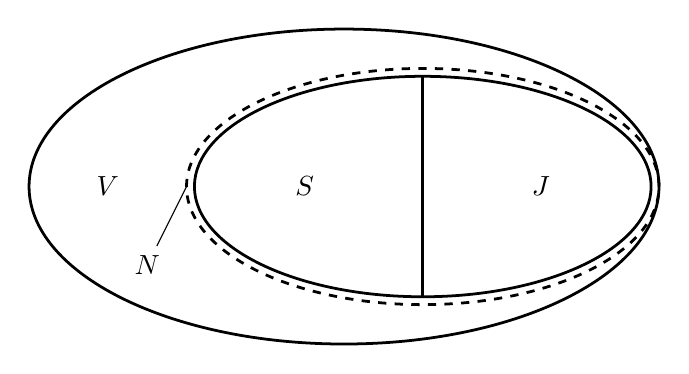
\begin{tikzpicture}
    \draw[l1] (0,0) circle [x radius = 4cm, y radius = 2cm];
    \draw[l1] (1,0) circle [x radius = 2.9cm, y radius = 1.4cm, line width=1];
    \draw[l1, dashed] (1,0) circle [x radius = 3cm, y radius = 1.5cm];
    \draw[l1] (1,1.4) -- (1,-1.4);
    \node at (-3, 0) {$\m{V}$};
    \node at (-.5, 0) {$\m{S}$};
    \node at (2.5, 0) {$\m{J}$};
    \node at (-2.5, -1) (nnode) {$\m{N}$};
    \draw (-2, 0) -- (nnode) ;
  \end{tikzpicture}
  \caption{The space occupied by the sets of vertices $\vset$ and nodes $\nset$ (union of syndrome-node set $\mathcal{S}$ and junction-node set $\mathcal{J}$).}\label{fig:sets}
\end{figure}

\begin{theorem}
  The set of nodes $\m{N} = \{n_1, n_2, .... n_{\nset}\}$ of cluster $C$ is a connected acyclic graph with root $n_r$, and exists next to the exists set of vertices $\m{V}$. The function of $\m{N}$ is to store the list of boundary edges at the nodes and to selectively bloom each node dependent on some calculated delay.
\end{theorem}


\section{Node parity and delay}\label{sec:nodedelay}

Even within the node set data structure of the cluster, the calculation of the PMW for each node is a heavy task. If done naively, the entire set needs to be traversed to find the PMW for every node in the set, and results to a quadratic complexity to the set size. Luckily, the node set data structure allows us to traverse the node set to compute the \emph{differential delay} of a node to its parent, and the \emph{root delay} after the set is fully traversed, which relates closely to the PMW. The delay computation complexity is linear to the set size.

\subsection{1D node tree}
To show how this calculation is performed, we first take the example of a 1D node tree $\nset_{1D}$ of size $S_\nset$ consisting of only syndrome-nodes $\sigma_i$, where all nodes lie on a horizontal line, but are allowed to grow in x and y directions (Figure \ref{fig:1dnodetree}). In our example, we only look at the first 3 nodes $n_0, n_1$ and $n_3$. The node tree continues after $n_2$ for $S_\nset - 3$ nodes.

\begin{figure}
  \centering
  \tikzstyle{nodea}=[node, minimum size=20, pattern=dots, pattern color=black!25!white]
  \tikzstyle{nodeb}=[nodel, solid, pattern=dots, pattern color=black!25!white]
  \begin{tikzpicture}
    \node at (-1,1) {$\nset_{1D}$};
    \node[nodea] at (0,0) (n1) {$n_0$};
    \node[nodea] at (2,0) (n2) {$n_1$};
    \node[nodea] at (4,0) (n3) {$n_2$};
    \node[nodeb] at (6,0) (n4) {};
    \node[nodeb] at (7,0) (n5) {};
    \node[nodeb] at (8,0) (n6) {};
    \node[nodeb] at (9,0) (n7) {};
    \draw[l1]  (n1) -- (n2) -- (n3) -- (n4);
    \draw[l1, dotted] (n4) -- (n5) -- (n6) -- (n7);
    \draw[l1, decorate, decoration={brace, amplitude=5}] (n4.west) ++(0,-.4) node[inner sep=0] (r1) {} (n7.east) ++(0,-.4) -- (r1) node[midway, below=4pt] {$S_{nset} -3$};
    \draw[l1, decorate, decoration={brace, amplitude=5}] (n7.west) ++ (0,.4) node[inner sep=0] (r2) {} (n4.east) ++ (0.,.4) -- (r2) node[midway, above=4pt] {$k$};
  \end{tikzpicture}
  \caption{The 1D node tree $\nset_{1D}$, consisting of only syndrome-nodes $\sigma_i$. The first 3 nodes $n_0, n_1, n_3$ are labelled, but the node tree continues after $n_2$ for $S_\nset - 3$ nodes. The distance of the edges between $n_3$ and $n_{S_\nset-1}$ is $(n_3, n_{S_\nset-1})=k$.}\label{fig:1dnodetree}
\end{figure}

Recall that the size of the node $n.s$ is equal to the iterations it has grown, one half-edge per iteration. This means that if a merge with some other cluster occurs on a boundary edge of $n$, the weight of the matchings edges within the flower of $n$ is equal to $\floor{n.s/2}+1$ or. For a merge on $n_0$, we also add edge $(n_1,n_2)$ and some value $k$ corresponding to the weight of matching edges in the remainder of the cluster. Let us calculate the PMW values for each of nodes $n_0, n_1, n_2$.
\begin{eqnarray*}
% \nonumber % Remove numbering (before each equation)
  PMW(n_0) &=& \floor{n_0.s/2}+1 + (n_1,n_2) + k \\
  PMW(n_1) &=& \floor{n_1.s/2}+1 + (n_0,n_1) + (n_1,n_2)+ k \\
  PMW(n_2) &=& \floor{n_2.s/2}+1 + (n_0,n_1) +k
\end{eqnarray*}
By taking the difference in PMW values of a node $n_i$ and its parent $n_{i-1}$, we can compute the \emph{differential delays} $\delta(n_i.d)$.
\begin{eqnarray*}
% \nonumber % Remove numbering (before each equation)
  \delta(n_1.d) &=& PMW(n_1.d) - PMW(n_0.d) \\
  \delta(n_2.d) &=& PMW(n_2.d) - PMW(n_1.d)
\end{eqnarray*}
The values of $n_i.d$ is thus dependent on the value of the root $n_0.d$, which can be any arbitrary value as the delay in the root is unknown when the calculation is initiated. For this reason, we call $n_i.d$ the \emph{root delays}, as it is the delay with respect to the root. To shorten, root delays are simply referred to as \emph{delays}.
\begin{eqnarray*}
% \nonumber % Remove numbering (before each equation)
  n_1.d &=& PMW(n_1) - PMW(n_0) + n_0.d = 2(\floor{n_1.s/2} - \floor{n_0.s/2} + (n_0,n_1)) + n_0.d \\
  n_2.d &=& PMW(n_2) - PMW(n_1) + n_1.d = 2(\floor{n_2.s/2} - \floor{n_1.s/2} - (n_1,n_2)) + n_1.d
\end{eqnarray*}
These delay values are not entirely correct, as $n_1.s = n_2.s = 2i$ yields the same value as  $n_1.s = 2i$, $n_2.s = 2i + 1$. We introduce growth support of a node $n.g = n.s \bmod 2$ to accommodate for this degeneracy in PMW, and add this to the delay values.
\begin{eqnarray*}
% \nonumber % Remove numbering (before each equation)
  n_1.d &=& 2\big(\floor{(n_1.s+n_1.g)/2} - \floor{(n_0.s+n_1.g)/2} + (n_0,n_1)\big) - (n_0.g + n_1.g)\bmod 2 + n_0.d \\
  n_2.d &=& 2\big(\floor{(n_2.s+n_2.g)/2} - \floor{(n_1.s+n_2.g)/2} - (n_1,n_2)\big) - (n_2.g + n_1.g)\bmod 2 + n_1.d
\end{eqnarray*}
If we were to consider some nodes $n_3, n_4...$ as well, we would find a trend in which the delay calculation is dependent on the \emph{parity} of the node number $i$. The delay of odd node $n_{2i+1}$ has the positive addition of $(n_{2i}, n_{2i+1})$ in its delay value, and the substraction of $(n_{2i-1}, n_{2i})$ for an even node $n_{2i}$. Thus we can generalize the delay calculation as the following:
\begin{multline}\label{eq:1ddelay}
n_i.d = n_{i-1}.d + 2\bigg(\floor{\frac{(n_i.s+n_i.g)}{2}} - \floor{\frac{(n_{i-1}.s+n_i.g)}{2}} + (-1)^{i+1}(n_{i-1}, n_i)\bigg) \\
         - (n_{i}.g + n_{i-1}.g)\bmod 2 \hspace{.5cm} | \hspace{.5cm} n_0.d = 0.
\end{multline}

Using equation \eqref{eq:1ddelay}, we can calculate all the relative delays in the 1D tree by traversing the node tree just once from left to right, where the initial delay is for example set to $n_0.d=0$. The difference between the root delays and the minimal root delay value in the cluster relates to the PMW.
\begin{equation}\label{eq:pmw}
  PMW(n_i) = n_i.d - \min \{n_0.d,...,n_{S_\nset-1}.d\} + K - n.w
\end{equation}
Here, the constant $K$ is equal to the lowest PMW in the cluster. Recall from theorem \ref{th:balancedbloom} that the algorithm searches for the lowest PMW nodes in the cluster, thus the value of $K$ is irrelevant for our algorithm. The variable $n.w$ stores the number of iterations a node has waited based on its calculated delay value, which is equivalent to the queue in lemma \ref{lem:calconce}, and will be clarified in \ref{sec:growingcluster}. If we store the minimal delay value in the cluster at the cluster object with
\begin{equation}\label{eq:cd}
  C.d = \min \{n_0.d,...,n_{S_\nset-1}.d\},
\end{equation}
we can define a \emph{Potential Normalized Weight} (PNW) that is normalized in $K$,
\begin{equation}\label{eq:pnw}
  PNW(n_i) = n_i.d - C.d - n.w.
\end{equation}
Balanced bloom in a cluster is now achieved by blooming the nodes that has $PNW(n_i) = 0$. Additionally, we can define a normalized delay (ND) of a node that is equal to the actual number of iterations for a node to wait:
\begin{equation}\label{eq:ad}
  ND(n_i) = n_i.d - C.d.
\end{equation}

\subsection{Node tree parity}

The 1D node tree does not accurately represent node trees that occupy a real lattice. On a 2D (Pauli errors) and 3D lattice (Pauli and measurement errors), the node tree is allowed to form in the same dimensions. As $\nset$ is an acyclic graph, the 3D variant can be considered equal to the 2D variant. The difference is that now the \emph{ancestry} in the tree, the set of parent-child relations, is not determined by some node number $i$, and each node can have more than 2 connections.

The delay calculation is done comparatively with the previous node, which means that there must be some directed path within $\nset$, such that there is a clear direction to traverse the tree for the delay calculation. We can start the calculation from the root $n_r$. The node parity, previously determined by the node number $i$, is now set by the number of children nodes modulo 2. To calculate this parity for each node without traversing all children nodes, we can use the following function
\begin{equation}\label{eq:nodeparitypart}
  n_\beta.p =
  \begin{cases}
    0, & \mbox{if $n_\beta$ has no children}  \\
    \big( \sum_{j} 1-n_{\gamma,j}.p \big ) \bmod 2 \hspace{.2cm} | \hspace{.2cm} \forall n_\gamma \mbox{ child of } n_\beta, & \mbox{otherwise},
  \end{cases}
\end{equation}
where $n_\beta$ is the node of interest, and each of the nodes $n_{\gamma,j}$ is a child of $n_\beta$. As this requires the parity of each child node to be known, the node parities of the entire set can be calculated by a depth-first search (DFS) of the node tree, and traversing back to the root recursively and applying the above equation.

\tikzstyle{odd}=[node1, dashed, pattern=dots, pattern color=black!25!white]
\tikzstyle{even}=[node1, pattern=dots, pattern color=black!25!white]
\tikzstyle{undef}=[node1, dotted, pattern=dots, pattern color=black!25!white]
\begin{figure}
  \centering
  \begin{tikzpicture}
    \node at (1,-1) {\emph{a)} $n_r = n_0$};
    \node[even] (0) at (1, 3) {$n_0$};
    \node[odd] (1) at (1, 2) {$n_1$};
    \node[odd] (2) at (1, 1) {$n_2$};
    \node[even] (3) at (1, 0) {$n_3$};
    \node[even] (4) at (0, 1) {$n_4$};
    \node[even] (5) at (0, 0) {$n_5$};
    \node[odd] (6) at (2, 2) {$n_6$};
    \node[even] (7) at (2, 1) {$n_7$};
    \node[even] (8) at (2, 0) {$n_8$};
    \draw[l1] (0) -- (1) -- (2) -- (3);
    \draw[l1] (1) -- (4); \draw[l1] (2) -- (5); \draw[l1] (2) -- (8);
    \draw[l1] (0) -- (6) -- (7);

    \begin{scope}[shift={(5,0)}]
      \node at (1,-1) {\emph{b)} $n_r = n_1$};
      \node[even] (1) at (1,3) {$n_1$};
      \node[even] (4) at (0, 2) {$n_4$};
      \node[odd] (2) at (1, 2) {$n_2$};
      \node[even] (3) at (1, 1) {$n_3$};
      \node[even] (5) at (0, 1) {$n_5$};
      \node[even] (8) at (2, 1) {$n_8$};
      \node[even] (0) at (2, 2) {$n_0$};
      \node[odd] (6) at (3, 1) {$n_6$};
      \node[even] (7) at (3, 0) {$n_7$};
      \draw[l1] (3) -- (2) -- (1) -- (0) -- (6) -- (7);
      \draw[l1] (4) -- (1); \draw[l1] (2) -- (5); \draw[l1] (2) -- (8);
    \end{scope}

    \begin{scope}[shift={(10,0)}]
      \node at (1,-1) {\emph{c)} $n_r = n_4$};
      \node[even] (4) at (1, 3) {$n_4$};
      \node[odd]  (1) at (1, 2) {$n_1$};
      \node[odd] (2) at (1, 1) {$n_2$};
      \node[even] (5) at (0, 0) {$n_5$};
      \node[even] (3) at (1, 0) {$n_3$};
      \node[even] (8) at (2, 0) {$n_8$};
      \node[even] (0) at (2, 1) {$n_0$};
      \node[odd] (6) at (3, 0) {$n_6$};
      \node[even] (7) at (3, -1) {$n_7$};
      \draw[l1] (7) -- (6) -- (0) -- (1) -- (2) -- (3);
      \draw[l1] (4) -- (1); \draw[l1] (2) -- (5); \draw[l1] (2) -- (8);
    \end{scope}
  \end{tikzpicture}
  \caption{The nodes in a node set can have even (solid) or odd (dashed) parities. The node parities are dependent on which node is set as root $n_r$. Here the same node tree $\nset$ is illustrated with different roots.}\label{fig:parities}
\end{figure}

Since $\nset$ is acyclic, any node in the set can be set as the root $n_r$ of the set, and the calculation of the parity would still be valid, although not identical. The node set $\nset$ is therefore a $semi$-directed tree, in which the edges are undirected, but an ancestry is set by the root node $n_r$ (see Figure \ref{fig:parities}). If the root node changes to $n_{r}'$, the ancestry within the tree changes, and the node parities within the set become unknown, or \emph{undefined}, requiring a new calculation of a reversed DFS from $n_{r}'$.

\begin{lemma}\label{lem:anynoderoot}
  Any node $n_i \in \m{N}_\alpha$ is a valid root.
\end{lemma}

\begin{lemma}\label{lem:nodeCalcParity}
  The node parity $n_i.p$ is the number of children nodes of node $n_i$ modulo 2, and can be calculated via a reversed DFS from root $n_r$. If a new node is set as root $n_r'$, the ancestry in a set changes, and node parities and delays in the set become undefined.
\end{lemma}

\subsection{Node tree delay}

The delay equation \eqref{eq:1ddelay} can be altered by replacing the node number $i$ with some parent-child relationship between nodes, similarly to the parity calculation. To calculate the node delays within $\nset$, we need to traverse $\nset$ in a second DFS from root $n_r$ with
\begin{multline}\label{eq:2ddelay}
  n_\beta.d = n_\alpha.d + 2\bigg(\floor{\frac{(n_\beta.s+n_\beta.g)}{2}} - \floor{\frac{(n_\alpha.s+n_\beta.g)}{2}} + (-1)^{n_\beta.p-1+1}(n_\alpha,n_\beta)\bigg) \\
         - (n_\beta.g + n_\alpha.g)\bmod 2 \hspace{.5cm} | \hspace{.5cm} n_r.d = 0, \hspace{.2cm} n_\beta \mbox{ child of } n_\alpha,
\end{multline}
where $n_\beta$ is the node of interest and $n_\alpha$ is an ancestor of $n_\beta$, and the sign of the edge component is now dependent on the node parity $n.p$. As the node parities are only defined while the same node is root per lemma \ref{lem:nodeCalcParity}, the delay calculation is only valid if the DFS is performed from the same root $n_r$ as in the parity calculation.

\begin{lemma}\label{lem:nodecalc_ancestrypath}
 The calculation of node delays is only valid while node parities within the set are defined along the same ancestry as the node delay calculation.
\end{lemma}

An interesting aspect of the node delays is that the differential delays $\delta(n.d)$ are indifferent for which node is set as root $n_r = n$. The root delay value $n.d$ however may differ for different roots as de delay value for the root node is arbitrary. But as we subtract by the minimal delay $C.d$ to find the normalized delay, the root dependance of node PMW and node PNW is accounted for. This fact strengthens lemma \ref{lem:anynoderoot}.

\subsection{Junction node parity and delay}

Up until now, the existence of junction-nodes has been neglected in the node parity and delays calculations. But as junction-nodes have the same properties as syndrome-nodes, junction-nodes can be delayed as well, and they must be included in the parity and delay calculations. Furthermore, without junction-nodes, lemma \ref{lem:anynoderoot} cannot be true for a node set $\nset$ for all nodes $n \in \nset$ for the same set of edges $\{\epsilon\}$.
\tikzstyle{junction}=[diamond, inner sep=1]
\begin{figure}
  \centering
  \begin{tikzpicture}
    \node[even] at (0,5) (0) {$\sigma_0$};
    \node[odd] at (0,4) (1) {$\sigma_1$};
    \node[even] at (0,3) (2) {$\sigma_2$};
    \node[odd] at (0,2) (3) {$\sigma_3$};
    \node[even] at (0,1) (4) {$\sigma_4$};
    \draw[l1] (0) -- (1) -- (2) -- (3) -- (4);
    \node[left=1 of 0] {$\nset_e$};
      \begin{scope}[shift={(6,0)}]
        \node[even] at (0,5) (0) {$\sigma_0$};
        \node[odd,junction] at (0,4) (1) {$j_1$};
        \node[odd] at (0,3) (2) {$\sigma_2$};
        \node[even,junction] at (0,2) (3) {$j_3$};
        \node[even] at (0,1) (4) {$\sigma_4$};
        \draw[l1] (0) -- (1) -- (2) -- (3) -- (4);
        \node[left=1 of 0] {$\nset_e'$};
      \end{scope}
  \end{tikzpicture}
  \caption{Two example node sets $\nset_e$ and $\nset_e'$ each containing 5 nodes, where syndrome-nodes $\sigma_i$ are circles and junction-nodes $j_i$ are diamonds. Their appropriate parities are calculated where an even parity correspond to continuous lines and odd to dashed lines. }\label{fig:junctionparity}
\end{figure}
As a junction-node is also allowed to bloom, similarly to a syndrome-node, equation \eqref{eq:2ddelay} still holds for junction-nodes. However, the parity of a junction-node is calculated differently. Consider an example node set $\nset_e$ with 5 syndrome-nodes $\{\sigma_1,...,\sigma_5\}$ lined up linearly with distance 1 between them and $n_r = \sigma_1$. Let us drop the $n.s, n.g$ components of the delay in equation \eqref{eq:2ddelay} as we are now only interested in the parity component $(-1)^{n_\beta.p-1+1}(n_\alpha, n_\beta)$. The parity of $\sigma_4$ is odd, therefore
\begin{equation*}
  \sigma_4.d = \sigma_3.d + 2(\sigma_3, \sigma_4).
\end{equation*}

Consider now a second example node set $\nset_e'$ with 3 syndrome-nodes and 2 junction-nodes $\{\sigma_1, j_2, \sigma_3, j_4, \sigma_5\}$. The PMW's for $\sigma_3$ and $j_4$ are $(\sigma_1, j_2) + (j_4, \sigma_5)$ and  $(\sigma_1, j_2) + (\sigma_3, j_4) + (j_4, \sigma_5)$, respectively, where the delay in $j_4$ is now
\begin{equation*}
  j_4.d = \sigma_3.d - 2(\sigma_3, j_4).
\end{equation*}
The edge component of the delay calculation now has an opposite sign. This flip in sign is due to a flip in node parity for junction-nodes compared to syndrome-nodes. As a result, we can generalize the parity calculation of equation \eqref{eq:nodeparitypart} for node sets including both syndrome-nodes and junction-nodes.
\begin{equation}\label{eq:nodeparity}
  n_\beta.p =
  \begin{cases}
    0, & \mbox{if $n_\beta$ has no children}  \\
    \big( \sum_{j} 1-n_{\gamma,j}.p \big ) \bmod 2 \hspace{.2cm} | \hspace{.2cm} \forall n_\gamma \mbox{ child of } n_\beta, & n_\beta \equiv \sigma_\beta \\
    1 - \big( \sum_{j} 1-n_{\gamma,j}.p \big ) \bmod 2 \hspace{.2cm} | \hspace{.2cm} \forall n_\gamma \mbox{ child of } n_\beta, & n_\beta \equiv j_\beta
  \end{cases}
\end{equation}

To put this into perspective of lemma \ref{lem:nodeCalcParity}, the parity of a syndrome-node is the number of children \emph{syndrome}-nodes. The parity of a junction-node is 1 minus the number of children syndrome-nodes. From here, our definitions of parity and delay calculation stay unchanged; the parities can to be calculated by a reversed DFS of the node tree from the root with equation \eqref{eq:nodeparity}, and the delays by a second DFS with equation \eqref{eq:2ddelay}.

\begin{lemma}\label{lem:nodecalc_junction}
  The node parity in a syndrome-node $\sigma.p$ is the number of children syndrome-nodes $\sigma_\gamma$ modulo 2. The node parity in junction-node $j.p$ is 1 minus the above definition.
\end{lemma}

\subsection{Parity and delay calculations}

With equation \eqref{eq:nodeparity} and \eqref{eq:delayequation}, we now finally have the tools to formulate the algorithms to calculate the node parities and delays. For a node set with root $n_r$, we can calculate the parities by calling the \emph{head recursive} function \codefunc{CalcParity} on $n_r$ in algorithm \ref{al:calcparity}, where we do a reverse DFS of the node tree. The node delays are calculated by calling the \emph{tail recursive} function \codefunc{CalcDelay} in algorithm \ref{al:calcdelay}, where we perform a second DFS of the node tree. These Parity and Delay Calculation will from this point be referred to as the PDC. Note that in the \codefunc{CalcDelay} algorithm, we have replaced the delay equation \eqref{eq:2ddelay} with equation \eqref{eq:delayequation}, which we will cover in the next section.

\begin{algo}[algotitle=CalcParity, label=al:calcparity]
\begin{algorithm}[H]
\SetKwData{node}{node}
\SetKwData{cluster}{cluster}
\SetKwData{child}{child}
\SetKwData{parity}{parity}
\SetKwData{pary}{p}
\SetKwFunction{cp}{CalcParity}
\SetKwFunction{summation}{Sum}

\KwData{\node}
\KwResult{Defined parities for all children of \node}

\BlankLine

\parity $=$ \summation{$[1 - $ \cp{\child} $\forall$ \child of \node $]$} $\%2$\;
\uIf{\node $\equiv \sigma$}{
    \node.\pary $=$ \parity}
\uElseIf{\node $\equiv j$}{
    \node.\pary $= 1-$ \parity}
\KwRet{\node.\pary}
\end{algorithm}
\end{algo}

\begin{algo}[algotitle=CalcDelay, label=al:calcdelay]
\begin{algorithm}[H]
\SetKwData{node}{node}
\SetKwData{cluster}{cluster}
\SetKwData{child}{child}
\SetKwData{delay}{d}
\SetKwFunction{cdelay}{CalcDelay}

\KwData{\node, \cluster}
\KwResult{Defined parities for all children of \node}

\BlankLine

\If{\node has an ancestor}{
  calculate \node.\delay with equation \eqref{eq:delayequation}\;
  \If{\node.\delay $<$ \cluster.\delay}{
    \cluster.\delay $=$ \node.\delay
    }
  }
\For{\child of \node}{
  \cdelay{\child, \cluster}
}
\end{algorithm}
\end{algo}
\begin{theorem}
  To prepare a cluster with node set $\m{N}$ and node root $n_r$ with undefined node parities and delays, we calculate node parities in $\m{N}$ by calling the head recursive function $\codefunc{CalcParity}(n_r)$, and sequentially calculate node delays in $\m{N}$ by calling the tail recursive function $\codefunc{CalcDelay}(n_r)$.
\end{theorem}

\begin{figure}
  \centering
  \begin{tikzpicture}[x=1.5cm,y=1.5cm]
    \node[node1,even] (a) at (1, 3) {$n_r$};
    \node[node1,odd]  (b) at (1, 2) {};
    \node[node1,odd]  (c) at (1, 1) {};
    \node[node1,even] (d) at (1, 0) {};
    \node[node1,even] (e) at (0, 1) {};
    \node[node1,even] (f) at (0, 0) {};
    \node[node1,odd]  (g) at (2, 2) {};
    \node[node1,even] (h) at (2, 1) {};
    \node[node1,even] (i) at (2, 0) {};
    \draw[l1] (a) -- (b) -- (c) -- (d);
    \draw[l1] (b) -- (e);
    \draw[l1] (c) -- (f);
    \draw[l1] (c) -- (i);
    \draw[l1] (a) -- (g) -- (h);

    \draw[l1, ->, dashed, color=cyan] (0, 1.3) -- +(45:0.85) arc (-45:0:.5) -- +(90:.6);
    \draw[l1, ->, dashed, color=cyan] (0, 0.3) -- +(45:0.85) arc (-45:0:.5) -- +(90:.2);
    \draw[l1, ->, dashed, color=cyan] (0.75,0.2) -- +(90:.3);
    \draw[l1, ->, dashed, color=cyan] (1.5,0.2) -- +(135:.4);
    \draw[l1, ->, dashed, color=cyan] (1.75,1.2) -- +(90:0.5) arc (0:45:.5) -- +(135:0.4);
    \draw[l1, ->, color=magenta] (1.4, 3) -- +(-45:1.1) arc (45:0:0.5) -- +(-90:0.7);
    \draw[l1, ->, color=magenta] (1.3, 2.1) -- +(-90:0.9) arc (180:225:.5) -- +(-45:0.7);
    \draw[l1, ->, color=magenta] (0.6, 1.3) -- +(225:.3);
    \draw[l1, ->, color=magenta] (0.6, 0.3) -- +(225:.3);
    \draw[l1, ->, color=magenta] (1.3, 0.3) -- +(-90:.2);
    \node[text=cyan] at (0,2.2) {Parity};
    \node[text=magenta] at (2.6,2.8) {Delay};
    \node at (0,3) {$\mathcal{N}$};
  \end{tikzpicture}
  \caption{The parity and delay calculation (PDC) performed on a the root node $n_r$, which is equivalent to two depth-first searches on $\mathcal{N}$ to compute node parities (head recursively) and delays (tail recursively).}\label{fig:2dfs}
\end{figure}

\subsection{BB-state optimization}\label{sec:bbstate}
In this section, we alter the delay equation \eqref{eq:2ddelay} with an extra parameter $f_{bloom}$ to optimize a trade-off in the Balanced Bloom algorithm. In the PDC, the appropriate delays in nodes are calculated such that, if the bloom in these nodes are delayed a number of iteration equal to the calculated delays, the PNW for every node in the set is zero. We will see how to grow a node set and how to join node sets in the following sections. But before we move on, there is one final problem with the delay calculation.

If some odd number of nodes $\nset^o$ is attached to $n^e$ of $\nset^e$ during an union of two node sets, node parities for nodes in subset $'\nset^e= \{n_i \in \nset^e | n_i \mbox{ ancestor of } n^e\}$ are flipped, where odd nodes become even and even become odd, which is called \emph{parity inversion}. Per lemma \ref{lem:nodeCalcParity} and \ref{lem:nodecalc_ancestrypath}, the delays in $'\nset^e$ are now undefined and need to be recalculated. Before the union, the cluster of $'\nset^e$ is grown according to Balanced Bloom, where the odd nodes are delayed and consequently the even nodes will have some node sizes larger than the odd node sizes $n^e_{even}.s > n^e_{odd}.s$.
After the union, the parities for nodes in $'\nset^e$ flip, and the pre-union even nodes are now odd and have some positive delay. As $n^e_{even}.s > n^e_{odd}.s$, the absolute delays (equation \eqref{eq:ad}) of these nodes are larger than the absolute delays of the pre-union odd nodes per equation \eqref{eq:2ddelay}. Subsequent parity inversions further increases the absolute delays in the post-union odd nodes.

To better illustrate this problem, we introduce the concept of the \emph{BB-state} $(M:I)$ of a cluster, where $M$ is equal to the maximum absolute delay in the cluster, and $I\leq M$ is the number of iterations grown while zero PNW in the cluster has not been reached. For example, a cluster with $M=4$ requires 4 growth iterations to reach zero PNW in all nodes in the cluster. The BB-state thus gives us an indication of the how near Balanced Bloom a cluster performs. Let the fraction $f=I/M$ be the \emph{balance factor}, then $f \to 1$ is equivalent to a larger degree of balanced PNW's and thus improves the heuristic for minimum-weight.
\begin{lemma}\label{lem:bbstate}
  The BB-state $(M:I)$ describes the degree of difference in PMW in the cluster, where the balance factor $f=I/M=1$ is equivalent to equal PMW.
\end{lemma}
In the context of the BB-state, the delayed bloom of odd nodes in cluster growth is equivalent to increasing the value of $I$. Once $f=1$ is reached after $I=B$ iterations, all nodes have zero PNW and none are delayed during further growth. As $f\to1$ increases the difference between even and odd node sizes, the balance factor at the moment of union $f_u$ is proportional to the increase in the value of $M$ after union or the fraction of the after-union $M_{AC}$ and before-union $M_{BC}$:
\begin{equation}\label{eq:bbpropto}
  f_u \propto \frac{M_{AU}}{M_{BU}} \geq 1.
\end{equation}
Subsequent parity inversions cause a gradual but certain increase in $M$ of the BB-state, depending on $f_u$ during the parity inversion at the union, requiring a growing number of growth iterations $I$ to reach the balanced BB-state $(M:M)$. Furthermore, as the lattice size is increased, the total number of unions of a cluster with other clusters also increases, leading to a growing number of parity inversions. Thus increasing the lattice size has the consequence that more growth iterations $I$ are needed to reach a balanced BB-state.
\begin{figure}
  \centering
    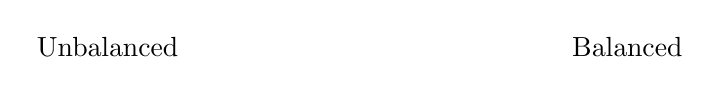
\begin{tikzpicture}
      \DSPECTRUM{4}{2}{1}
      \draw (-1.5,.5) node[align=right] {Unbalanced} ++(6.6,0) node[align=left] {Balanced};
    \end{tikzpicture}
  \caption{Visual representation of the BB-state $(4:2)$. The size of the full x-axis is $M=4$ and the length of the bar is $I=2$. The left side of the spectrum is equivalent to the unbalanced BB-state, and the right the balanced state.}\label{fig:bbstate}
\end{figure}

This is a trade-off in the effectiveness of Balanced Bloom. On the one hand, it is preferred that $f\to1$ to reach a balanced BB-state, but on the other, $f$ is also proportional to the number of iterations needed to actually reach $f=1$ in the case of parity inversions. To this end, we introduce the balance constant $f_{bloom}$ to equation \eqref{eq:2ddelay}.
\begin{multline}\label{eq:delayequation}
  n_\beta.d = n_\alpha.d + \Bigg \lceil f_{bloom} \Bigg( 2\bigg(\floor{\frac{(n_\beta.s+n_\beta.g)}{2}} - \floor{\frac{(n_\alpha.s+n_\beta.g)}{2}} + (-1)^{n_\beta.p-1+1}(n_\alpha,n_\beta)\bigg)
   \Bigg) \\ - (n_\beta.g + n_\alpha.g)\bmod 2 \Bigg \rceil \hspace{.3cm} | \hspace{.3cm} n_r.d = 0, \hspace{.2cm} n_\beta \mbox{ child of } n_\alpha, \hspace{.2cm} f_{bloom} \in [0, 1]
\end{multline}
\begin{lemma}\label{lem:tradeoff}
  The balance factor $f$ is the cause of a trade-off of Balanced Bloom, where $f\to1$ during growth improves the heuristic for minimum-weight, but also increases the number of growth iterations needed to reach $f=1$.
\end{lemma}

\tikzstyle{edge}=[above,midway,font=\tiny]
\newcommand\DLINE[4]{
  \draw (#1, #2) ++ (-.3,-.9) node[inner sep=0] (lb) {} ++(#3,0) ++(.6,0) node[inner sep=0] (rb) {} ++(0,0.4) node[inner sep=0] (rt) {};;
  \path[fill=white!80!black, rounded corners=2pt] (lb) rectangle (rt);
  \ifnumequal{#4}{1}{\draw[thin] (lb) -- (rb);}{}
}
\begin{figure}
\centering
    \begin{tikzpicture}[on grid, scale=1]
      \foreach \x in {0,3,6}{\DLINE{\x}{0}{2}{1}}
      \foreach \x in {0,2,3,5,6,8}{\draw (\x,0) node [even] (a\x) {1} ++(0,-.7) node (ad\x) {0};}
      \foreach[count=\i] \x in {1,4,7}{      \draw (\x,0) node [odd]  (a\x) {1} ++(0,-.7) node (ad\x) {2};
                                             \node at (\x,0.7) {$\nset_\i$};}
      \foreach \x in {0.5,3.5,6.5}{\DSPECTRA{2}{0}{\x}{-1.5}{0.3}{0.5}}
      \draw[l1] (a0) -- (a1) node[edge]{1} -- (a2) node[edge]{1} (a3) -- (a4) node[edge]{1} -- (a5) node[edge]{1} (a6) -- (a7) node[edge]{1} -- (a8) node[edge]{1};

      \begin{scope}[shift={(0,-3)}]
      \foreach \x in {0,3,6}{\DLINE{\x}{0}{2}{0}}
      \foreach \x in {0,2,3,5,6,8}{\draw (\x,0) node [even] (e\x) {2} ++(0,-.7) node {0};}
      \foreach \x in {1,4,7}{      \draw (\x,0) node [odd]  (e\x) {1} ++(0,-.7) node {1};}
      \foreach \x in {0.5,3.5,6.5}{\DSPECTRA{2}{1}{\x}{-1.5}{0.3}{0.5}}
      \draw[l1] (e0) -- (e1) node[edge]{1} -- (e2) node[edge]{1} (e3) -- (e4) node[edge]{1} -- (e5) node[edge]{1} (e6) -- (e7) node[edge]{1} -- (e8) node[edge]{1};
      \draw[l1, dashed] (e2) -- (e3) (e5) -- (e6);
      \end{scope}

      \begin{scope}[shift={(0,-6)}]
      \DLINE{0}{0}{8}{1}
      \foreach \x in {0,2,6,8}{\draw (\x,0) node [even] (b\x) {2} ++(0,-.7) node {0};}
      \foreach \x in {1,7}{    \draw (\x,0) node [odd]  (b\x) {1} ++(0,-.7) node {1};}
      \foreach \x in {3,5}{    \draw (\x,0) node [odd]  (b\x) {2} ++(0,-.7) node {4};}
                               \draw (4,0)  node [even] (b4)  {1} ++(0,-.7) node {1};
      \DSPECTRA{4}{0}{3}{-1.5}{0.3}{0.5}
      \draw[l1] (b0) -- (b1) node[edge]{1} -- (b2) node[edge]{1} -- (b3) node[edge]{2} -- (b4) node[edge]{1} -- (b5) node[edge]{1} -- (b6) node[edge]{2} -- (b7) node[edge]{1} -- (b8) node[edge]{1};
      \end{scope}

      \node at (-2,0) {$n_i.s$};
      \node at (-2,-0.75) {$n_i.d$};
      \node at (-2,-1.5) {$(M:I)$};
      \draw[semithick, ->] (9,-.75) to [out=-60, in=60] ++(0,-2.5);
      \draw[semithick, ->] (9,-3.75) to [out=-60, in=60] ++(0,-2.5);
      \node at (10, -2) [align=right, text width = 3cm] {\underline{PDC}, \codefunc{Grow}};
      \node at (10, -5) [align=right, text width = 3cm] {\codefunc{Join}, \underline{PDC}};

%       \draw[l1, ->] (a8) ++(1,-.35) -- +(0,-2) node[midway, right, text width = 5cm, align=left] {Grow and calculate \\delay with eq. \eqref{eq:2ddelay}};
%       \draw[l1, ->] (c8) ++(1,-.35) -- +(0,-2) node[midway, right, text width = 5cm, align=left] {Grow and calculate \\delay with eq. \eqref{eq:delayequation},\\ $K_{bloom} = 0.5$};
    \end{tikzpicture}
    \caption{The delay values $n_i.d$ and the BB-states $(M:I)$ for 3 odd clusters $\{\nset_1, \nset_2, \nset_3\}$ of 3 nodes that grow and join into a size-9 cluster. Initially (top), PDC's are performed with delay equation \eqref{eq:2ddelay} on each odd cluster which have BB-states $(2:0)$, with delay $2$ in the middle node. The clusters are grown (middle), where the middle node is delayed, such that it's delay value decreases to $1$, and the clusters have B-states $(2:1)$. The clusters join (bottom) to a single odd cluster, which is selected for growth. Hence PDC is performed again, and the BB-state is $(4:0)$, thus requiring 4 growth iterations before zero PNW is reached in all nodes.}\label{fig:kbloom}
\end{figure}

\begin{figure}
  \centering
  \begin{tikzpicture}
      \foreach \x in {0,3,6}{\DLINE{\x}{0}{2}{1}}
      \foreach \x in {0,2,3,5,6,8}{\draw (\x,0) node [even] (c\x) {1} ++(0,-.7) node {0};}
      \foreach[count=\i] \x in {1,4,7}{      \draw (\x,0) node [odd]  (c\x) {1} ++(0,-.7) node (cd\x) {2};
                                             \node at (\x,0.7) {$\nset_\i$};}
      \foreach \x in {.75,3.75,6.75}{\DSPECTRA{1}{0}{\x}{-1.5}{0.3}{0.5}}
      \draw[l1] (c0) -- (c1) node[edge]{1} -- (c2) node[edge]{1} (c3) -- (c4) node[edge]{1} -- (c5) node[edge]{1} (c6) -- (c7) node[edge]{1} -- (c8) node[edge]{1};

      \begin{scope}[shift={(0,-3)}]
      \foreach \x in {0,3,6}{\DLINE{\x}{0}{2}{0}}
      \foreach \x in {0,2,3,5,6,8}{\draw (\x,0) node [even] (c\x) {2} ++(0,-.7) node {0};}
      \foreach \x in {1,4,7}{      \draw (\x,0) node [odd]  (c\x) {1} ++(0,-.7) node {0};}
      \foreach \x in {.75,3.75,6.75}{\DSPECTRA{1}{1}{\x}{-1.5}{0.3}{0.5}}
      \draw[l1] (c0) -- (c1) node[edge]{1} -- (c2) node[edge]{1} (c3) -- (c4) node[edge]{1} -- (c5) node[edge]{1} (c6) -- (c7) node[edge]{1} -- (c8) node[edge]{1};
      \draw[l1, dashed] (e2) -- (e3) (e5) -- (e6);
      \end{scope}

      \begin{scope}[shift={(0,-6)}]
      \DLINE{0}{0}{8}{1}
      \foreach \x in {0,2,6,8}{\draw (\x,0) node [even] (d\x) {2} ++(0,-.7) node {0};}
      \foreach \x in {1,7}{    \draw (\x,0) node [odd]  (d\x) {1} ++(0,-.7) node {0};}
      \foreach \x in {3,5}{    \draw (\x,0) node [odd]  (d\x) {2} ++(0,-.7) node {2};}
                               \draw (4,0)  node [even] (d4)  {1} ++(0,-.7) node {0};
      \draw[l1] (d0) -- (d1) node[edge]{1} -- (d2) node[edge]{1} -- (d3) node[edge]{2} -- (d4) node[edge]{1} -- (d5) node[edge]{1} -- (d6) node[edge]{2} -- (d7) node[edge]{1} -- (d8) node[edge]{1};
      \DSPECTRA{2}{0}{3.5}{-1.5}{0.3}{0.5}
      \end{scope}

      \node at (-2,0) {$n_i.s$};
      \node at (-2,-0.75) {$n_i.d$};
      \node at (-2,-1.5) {$(M:I)$};
      \draw[semithick, ->] (9,-.75) to [out=-60, in=60] ++(0,-2.5);
      \draw[semithick, ->] (9,-3.75) to [out=-60, in=60] ++(0,-2.5);
      \node at (10, -2) [align=right, text width = 3cm] {\underline{PDC}, \codefunc{Grow}};
      \node at (10, -5) [align=right, text width = 3cm] {\codefunc{Join}, \underline{PDC}};

  \end{tikzpicture}
  \caption{The same clusters, growths and joins as in Figure \ref{fig:kbloom}, but now with delay equation \eqref{eq:delayequation} for $f_{bloom} = 1/2$. With the redefined BB-state $(f_{bloom}M:I)$, $f=1$ can be reached in fewer growth iterations; e.g. after 1 round (middle), $(1:1)$ is reached. Also after join to a single cluster (bottom), fewer iterations are needed (2 compared to 4 in Figure \ref{fig:kbloom}).}\label{fig:kbloom2}
\end{figure}
For any $f_{bloom} < 1$, a cluster will never actually reach the balanced BB-state, but only $(M:f_{bloom}I)$. Consequently, in the case of parity inversion, the difference in node sizes between even and odd nodes is decreased, such $f\to f_{bloom}$ can be reached in a lower number of growth iterations. Alternatively, the BB-state can be redefined as $(f_{bloom}M:I)$, where $f=1$ can now be reached in fewer growth iterations if $f_{bloom} <1$.  From intuition the balance constant should be around $f_{bloom} = 1/2$, which we will use in this thesis. For this value, the absolute delays in a node set are halved, such that both before and after the parity inversion, the lower halve of the BB-state spectrum of delays is occupied.
\begin{theorem}
  The degree of delay $f_{bloom} \in [0, 1]$ determines the factor of the calculated delays between the even and odd nodes. For any $f_{bloom} < 1$, a cluster will never reach zero PNW in the cluster, but only $f=I/M=f_{bloom}$, which also decreases the number of growth iterations needed to reach $f=f_{bloom}$ again after parity inversion.
\end{theorem}

The optimal value of $f_{bloom}$ is dependent on the number of parity inversions, and consequently the lattice size , bucket number $i$, and the cluster sizes $S_\nset, S_\vset$, such that $f\to1$ after the last parity inversion of a cluster is maximally occupied. We do not provide an analytical approach to estimate the optimal value of $f_{bloom}(L, i, S_\nset, S_\vset)$ here, but note that other values than $f_{bloom} = 1/2$ should be explored. \\

\section{Growing a cluster}\label{sec:growingcluster}
With the knowledge of previous section, we now have the equations and algorithms available to describe the steps to grow a cluster in the context of Balanced Bloom. In the node data structure, the growth of a cluster is equivalent to a DFS of the node set. The boundary list for each cluster is not stored at $C$, but separately stored at each of the nodes $n_i$ in $\m{N}$. We traverse all $n_i \in \m{N}$ from the root $n_r$ and apply $\codefunc{Bloom}(n_i)$, which increases the support of all boundary edges in $n_i.m{L}$ by 1.

Recall from theorem \ref{th:balancedbloom} that with Balanced Bloom, we need to conditionally bloom the nodes with minimal PMW, or zero PNW. Also, from lemma \ref{lem:calconce}, the delays are not recalculated after each growth iteration (in the absence of unions) but stored in memory at the nodes, and the PNW is updated via $n.w$ (equation \eqref{eq:pnw}), the number of growths a node has waited. Thus, we can define a function $\codefunc{Grow}(n_i)$ where $\codefunc{Bloom}(n_i)$ is only applied if $PNW(n_i) = n_i.d - C.d - n_i.w = 0$ is satisfied. If not, node $n_i$ is skipped, the wait is increased $n_i.w = n_i.w +1$ and \codefunc{Bloom} is recursively applied on its children.

New vertices $v_{new}$ grown from node $n_i$ are added to $\m{V}$, while storing the seed node at each new vertex $v_{new}.n = n_i$. New boundary edges are appended to the boundary list $n_i.\m{L}$ stored each seed node $n_i$. The number of nodes in $\m{N}$ and the shape of the flower bush tree therefore does not change while no merge between clusters has happened.

\begin{theorem}\label{the:grownode}
  A cluster $C$ is grown by calling $\codefunc{Grow}(n)$ on the root node $n_r$, which first checks for the wait of the current node $ n.d - C.d - n.w = 0$ to grow its boundary edges with $\codefunc{Bloom}(n)$, and then recursively applies \codefunc{Grow} to its children.
\end{theorem}

\begin{algo}[algotitle=Grow, label=al:bbgrow]
\begin{algorithm}[H]

\SetKwData{node}{node}
\SetKwData{child}{child}
\SetKwData{cluster}{cluster}
\SetKwData{delay}{d}\SetKwData{waited}{w}
\SetKwData{edge}{edge}\SetKwData{support}{support}
\SetKwFunction{grow}{Grow}
\SetKwFunction{bloom}{Bloom}

\KwData{\node}
\KwResult{A node that has either grown or waited one iteration.}

\BlankLine

\eIf{\node.\delay $-$ \cluster.\delay $-$ \node.\waited $=0$}{
  \bloom{\node}, add all edges \edge.\support $= 2$ to $\m{F}$
}{
  \node.\waited $+=1$
}
\For{\child of \node}{
  \grow{\child}
}

\end{algorithm}
\end{algo}


\section{Joining node sets}\label{sec:jointnodesets}
With the extension of the node set data structure, during a union of clusters $C_\alpha$ and $C_\beta$, we have to additionally combine the node sets $\m{N}_{\alpha}$ and $\m{N}_\beta$ that requires its own set of rules that we will explain in this section. Let us first make a clear distinction between the various routines. On the vertex set $\m{V}$ we apply $\codefunc{Union}(v^\alpha, v^\beta)$, on the two vertices spanning the edge connecting two clusters. On node set $\m{N}$, we introduce here $\codefunc{Join}(n^\alpha, n^\beta)$, which is called on the two nodes $n^\alpha, n^\beta$ that seed vertices $v^\alpha, v^\beta$, respectively. During a merge of two clusters, these routines are both applied on their respective sets. From this point, when either one of the expressions "merge clusters $C^\alpha$ and $C^\beta$", "the union of vertex sets $\m{V}_\alpha$ and $\m{V}_\beta$" or the "join of node sets $\m{N}_{\alpha}$ and $\m{N}_\beta$" is mentioned, it is always implied that both routines are executed.

Within the vertex set $\m{V}$, we apply \emph{path compression} and \emph{weighted union} to minimize the depth of the tree and therefore minimizing the calls to the \codefunc{Find} function. Similarly, in the node set $\m{N}$, we would also like to apply a set of rules to minimize the calls to \codefunc{CalcParity} and \codefunc{CalcDelay}, which are the parity and delay calculation(s) (PDC). As the structure of the tree is crucial in computing the parity of the nodes and relative delays between the nodes, these rules will be quite different than in vertex set $\m{V}$ that changes the ancestry dynamically by path compression. Join rules will be dependent on the parities of the joining node sets $\m{N}.p$, which is the number of syndrome-nodes in the set modulo 2. The parity of a node set $\m{N}.p$ is equivalent to the parity of a cluster $C.p$, which also refer to the number of syndromes in the cluster.
\begin{lemma}
  The parity of node set $\m{N}.p$ is the number of syndrome-nodes $a_i \in \m{N}$ modulo 2. The parity of node set $\m{N}.p$ is analogous to cluster parity $C.p$.
\end{lemma}

Only odd clusters with odd parity node sets are grown in the UF-decoder. It may thus be tempting to conclude that a join must include at least one odd node set. This is however not true as within the same growth iteration, there may be many joins, where some odd cluster $\nset_1^o$ first joins with odd cluster $\nset_2^o$, but also joins with even cluster $\nset_3^e$. The second join is effectively between even clusters. Hence there are 3 types of joins: 1) odd-odd, 2) even-odd and 3) even-even, where even-odd is equivalent to odd-even. These joins can be put into 2 \emph{classes}, dependent on the parity of the resulting cluster. Both odd-odd and even-even joins to an even cluster and thus belongs to the even class join (E-join), whereas even-odd (and odd-even) joins to an odd cluster in the odd class join (O-join).


\subsection{E-joins}

For E-joins, the joined even cluster $\nset^e$ will not be selected for growth by the UF-decoder. One could naively conclude that no PDC will be performed and no PDC minimization can be made. This is of course not true as it is entirely possible that another cluster grows, and merges with the cluster of $\m{N}^{e}$ in a O-join. In that case, we might think about "reusing" some of the node parities and delays that were already calculated in the subsets of $\m{N}^e$, such that $\m{N}^{e}$ doesn't have to be traversed entirely for its parities and delays. In this case, a \emph{partial PDC} is performed over the undefined part.

To reuse prior calculated parities and delays, we need to traverse $\nset^e$ to find which sections are still valid, and which sections are not. This is no trivial task and often requires us to traverse the entire set $\nset^e$, especially when the clusters in the E-join are the results of joins within the same growth iteration.  Checking the validity to reuse prior parities and delays then acquires the same complexity as redoing the PDC over the subset $\nset^e$. Hence the node parities and delays in the joined set after an E-join are \emph{undefined}.

\begin{lemma}\label{lem:nodecalc_even}
  Node parities and delays become undefined if multiple node sets joins into a new set $\m{N}$ with even parity.
\end{lemma}

\subsection{O-joins}

Consider now an O-join between an even node set $\m{N}^e$ and an odd node set $\m{N}^o$ in nodes $n^e, n^o$ respectively, and assume that this join is due to the growth of odd cluster $\m{N}^o$ onto an "idle" $\m{N}^e$. The join of these two sets produces a new odd node set $\m{N}_{new}^o$ with subsets $'\nset^e$ and $'\nset^o$, referring to the original node sets. We are provided with two choices, A) make $n^e$ child of $n^o$, or B) make $n^o$ child of $n^e$. The ancestry in the parent node set stays unchanged, but the ancestry in the child subset is changed by setting the joining node in the child set $n^c$ as the sub-root of the child subset $'\m{N}^c$. This is allowed per lemma \ref{lem:anynoderoot}, but removes any calculated parities or delays per lemma \ref{lem:nodeCalcParity} and \ref{lem:nodecalc_ancestrypath}.

For option A, an even number of nodes of $'\m{N}^e$ is attached to $n^o$, and the ancestry in $'\m{N}^o$ hasn't changed. The parities and delays in $'\m{N}^o$ stay valid and can be reused. From $n^e$, which is now the sub-root of  $'\m{N}^e$, a partial PDC is applied, where the relative delay of $n^e$ is calculated with respect to its parent $n^o$ (Figure \ref{fig:joinrules}A). This is efficient as the parities and delays in $'\m{N}^e$ are already undefined per lemma \ref{lem:nodecalc_even}. For option B, we need to redo the PDC in both $'\m{N}^o$ and $'\m{N}^e$ (Figure \ref{fig:joinrules}B), as $'\m{N}^o$ has a changed ancestry and  $'\m{N}^e$ is even. The PDC is thus minimized if option A is always chosen. \\

% If the subset $'\m{N}^e$ consists of only two odd node sub-subsets $''\m{N}^o_0, ''\m{N}^o_1$, where $n_0, n_1$ are the joining nodes, the ancestry in $''\m{N}^o_0$ is preserved and $n_1$ is the sub-root of $''\m{N}^o_1$. We see that the parities in all ancestors of $n_0$ are flipped. Let's consider the cases and find whether we can minimize the parity and delay calculation in $'\m{N}^{e}$.
%
% For case a), an even number of nodes of $'\m{N}^e$ is attached to $n^o$, and the ancestry in $'\m{N}^o$ hasn't changed. This means that the parities in $'\m{N}^o$ do not change per lemma \ref{lem:nodeCalcParity}, and the delays in $'\m{N}^o$ are still valid as per lemma \ref{lem:nodecalc_ancestrypath}. In $'\m{N}^e$, as the ancestry path has changed, we are certain to traverse $'\m{N}^e$ from the sub-root $n^e$ to calculate the delays in this subset which is in the order of $S_{'\m{N}^e}$.
%
% In case b), as an odd number of nodes of $'\m{N}^o$ is attached to $n^e$, it means that parities of all ancestor of $n^e$ are flipped. As the ancestry in $'\m{N}^{o}$ has changed, we are certain to traverse $'\m{N}^o$ from the sub-root $n^o$ to calculate the delays which is in the order of $S_{'\m{N}^o}$. The node parity changes in $'\m{N}^e$ will be dependent on the location of $n^e$ in the ancestry compared to $n^1$ and $n^2$, and all children nodes of these parity changes will have to recalculate their delays. Let's call the number of nodes needs to calculate parity and delays in $'\m{N}^e$ a value $S_e \leq S_{'\m{N}^e}$, leaving the total number of operations in the order of $S_e + S_{'\m{N}^o}$.
%
% For $'\m{N}^e$ consisting of two subsets, keeping track of the parity changes between $n^e$, $n^0$ and $n^1$ is still an easy task, and we might gain in minimization in operations in case b) compared to case a) for some value $S_e$ such that $S_e + S_{'\m{N}^o} < S_{'\m{N}^e}$. But as the number of subsets in $'\m{N}^e$ increases, the task of finding the ancestry paths of parity changes becomes analogous to traversing $'\m{N}^e$ entirely $S_e \rightarrow S_{'\m{N}^e}$. To simplify, we always choose case a.
The rules are thus very simple for the function $\codefunc{Join}(n^\alpha, n^\beta)$. For O-joins between an even and an odd node set $\nset^e, \nset^o$ in the nodes $n^e, n^o$, always make the even node set a child of the even node set, where $n^e$ is now the sub-root of the subset $'\nset^e$. For E-joins between two even or two odd node sets, the parent and child sets can be picked at random. Finally, we note the concept of a $partial$ PDC is rather redundant, as a PDC is always applied partially on the undefined part of a set for any set with $S_\nset>1$.

\begin{theorem}\label{the:nodejoint}
  The union of node sets $\m{N}^\alpha, \m{N}^\beta$ on nodes $n^\alpha, n^\beta$ respectively is performed with $\codefunc{Join}(n^\alpha, n^\beta)$. If the join is between an even and an odd node set $\nset^e, \nset^o$ in the nodes $n^e, n^o$, $\codefunc{Join}(n^e, n^o)$ makes the node of the even set $n^e$ a child of the node of the odd set $n^o$. If the join is between two even or two odd node sets, the choice is arbitrary.
\end{theorem}

\begin{figure}
\centering
\begin{tikzpicture}[on grid]
  \node (o1) [even] at (1.5, 1) {$n_1$};
  \node (o2) [even] at (1, 0) {$n_2$};
  \node (o3) [even] at (2, 0) {$n_3$};
  \node (e4) [undef] at (3.5,1) {$n_4$};
  \node (e5) [undef] at (3.5,0) {$n_5$};
  \draw[l1] (o2) -- (o1) -- (o3) (e4) -- (e5);
  \draw[l1, dashed] (o3) -- (e5) node[midway,below] (a) {};
  \draw[l1, <-] (a) -- ++(0,-.5) node[below] {$\codefunc{Join}(n_3, n_5)$};

  \begin{scope}[shift={(5,1)}]
  \node (o1) [even] at (1.5, 1) {$n_1$};
  \node (o2) [even] at (1, 0) {$n_2$};
  \node (o3) [even] at (2, 0) {$n_3$};
  \node (e4) [undef] at (2,-2) {$n_4$};
  \node (e5) [undef] at (2,-1) {$n_5$};
  \draw[l1] (o2) -- (o1) -- (o3) -- (e5) -- (e4);
  \draw[l1, ->, dashed, color=cyan] (e4) ++(-.7,0) -- + (0,1);
  \draw[l1, ->, color=magenta] (o3) ++(.7,-.5) -- +(0,-1.5);
  \end{scope}

  \begin{scope}[shift={(10,1.5)}]
  \node (o1) [even] at (1, -2) {$n_1$};
  \node (o2) [even] at (1, -3) {$n_2$};
  \node (o3) [even] at (1, -1) {$n_3$};
  \node (e4) [undef] at (1,1) {$n_4$};
  \node (e5) [undef] at (1,0) {$n_5$};
  \draw[l1] (o2) -- (o1) -- (o3) -- (e5) -- (e4);
  \draw[l1, ->, dashed, color=cyan] (o3) ++(-.7,.5) -- +(0,1.5);
  \draw[l1, ->, dashed, color=cyan] (o2) ++(-.7,0) -- +(0,2);
  \draw[l1, ->, color=magenta] (e4) ++(.7,0) -- +(0,-1);
  \draw[l1, ->, color=magenta](e5) ++(.7,-.5) -- + (0,-2.5);
  \end{scope}

  \node at (5,2) {A)};
  \node at (9.5,2) {B)};
\end{tikzpicture}
\caption{An odd cluster $\nset^e=\{n_1, n_2, n_3\}$ with root $n^e_r = n_1$ joins with an odd cluster $\nset^o=\{n_4, n_5\}$ with root $n^o_r=n^4$ on nodes $n_3, n_5$, respectively, to a new set $\nset$ with subsets $'\nset^e$ and $'\nset^o$. Here we use dotted outlines on the nodes of $'\nset^e$ to indicate that their parities and delays are undefined. If we choose to A), make $n_5$ a child of $n_3$, the parities and delays in $'\nset^o$ can be reused, and we only have to redo PDC over $'\nset^e$. If we choose to B), make $n_3$ a child of $n_5$, PDC's have to be redone over both $'\nset^o$, as it has a new sub-root $n_3$, as well as $'\nset^e$ as its parties and delays were undefined.}\label{fig:joinrules}
\end{figure}

\subsection{Prevention of redundant PDC's}\label{sec:multiplejoint}
The final rule for joins between clusters introduces a data structure to store undefined parts of a cluster, such that multiple PDC's over a subset is prevented. If there are many O-joins (and E-joins) within the same growth iteration $i$, that at the end of $i$ results to one single cluster $\nset$, every O-join will require the PDC over the even subset. There may be subsets where multiple PDC's are performed before the final cluster $\nset$ is constructed. If the PDC is done directly after an O-join, the calculated values may thus be redundant.

Consider an example with 5 odd clusters $\nset_1, ...,  \nset_5$ (Figure \ref{fig:redundantpdc}). The join of $\nset_1$ and $\nset_2$ to $\nset_{12}$ is an E-join and requires no PDC. The join of $\nset_{12}$ and $\nset_3$ is an O-join, and we apply PDC in $\nset_{12}$. The join of $\nset_{123}$ and $\nset_4$ is an E-join and the join of $\nset_{1234}$ and $\nset_5$ is an O-join, with PDC executed in $\nset_{1234}$. The earlier computation in $\nset_{12}$ was therefore unnecessary and possibly invalid.

\tikzstyle{enset}=[node1, thick, double, font=\footnotesize]
\tikzstyle{onset}=[node1, thick, densely dashed, double, font=\footnotesize]

\begin{figure}
\centering
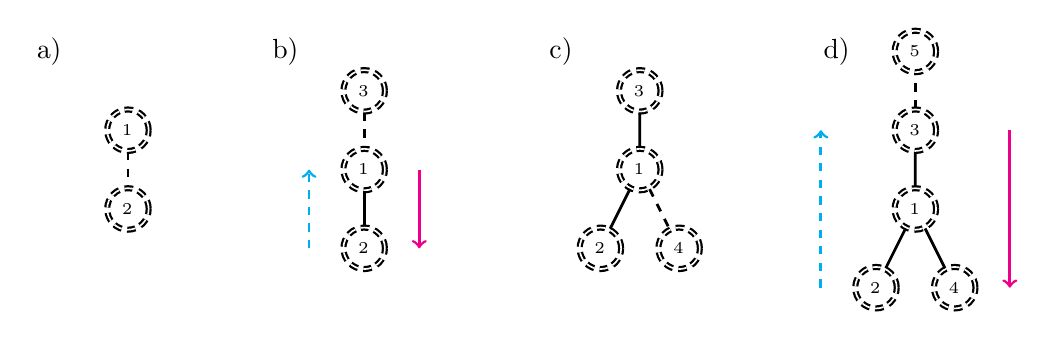
\begin{tikzpicture}
  \node (n1) [onset] at (0,0) {$\nset_1$};
  \node (n2) [onset] at (0,-1) {$\nset_2$};
  \draw[l1, dashed] (n1) -- (n2);

  \begin{scope}[shift={(3,-.5)}]
  \node (n3) [onset] at (0,1) {$\nset_3$};
  \node (n1) [onset] at (0,0) {$\nset_1$};
  \node (n2) [onset] at (0,-1) {$\nset_2$};
  \draw[l1, dashed] (n3) -- (n1); \draw[l1] (n1) -- (n2);
  \draw[l1, ->, dashed, color=cyan] (n2) ++(-.7,0) -- +(0,1);
  \draw[l1, ->, color=magenta] (n1) ++(.7,0) -- +(0,-1);
  \end{scope}

  \begin{scope}[shift={(6.5,-.5)}]
  \node (n3) [onset] at (0,1) {$\nset_3$};
  \node (n1) [onset] at (0,0) {$\nset_1$};
  \node (n2) [onset] at (-.5,-1) {$\nset_2$};
  \node (n4) [onset] at (.5,-1) {$\nset_4$};
  \draw[l1, dashed] (n1) -- (n4); \draw[l1] (n3) -- (n1) -- (n2);
  \end{scope}

  \begin{scope}[shift={(10,-1)}]
  \node (n5) [onset] at (0,2) {$\nset_5$};
  \node (n3) [onset] at (0,1) {$\nset_3$};
  \node (n1) [onset] at (0,0) {$\nset_1$};
  \node (n2) [onset] at (-.5,-1) {$\nset_2$};
  \node (n4) [onset] at (.5,-1) {$\nset_4$};
  \draw[l1, dashed] (n3) -- (n5); \draw[l1] (n3) -- (n1) -- (n2) (n1) -- (n4);
  \draw[l1, ->, dashed, color=cyan] (n2) ++(-.7,0) -- +(0,2);
  \draw[l1, ->, color=magenta] (n3) ++(1.2,0) -- +(0,-2);
  \end{scope}

  \node at (-1, 1) {a)};
  \node at (2, 1) {b)};
  \node at (5.5, 1) {c)};
  \node at (9, 1) {d)};
\end{tikzpicture}
\caption{If the PDC is directly performed on the even subset in an O-join, there may be redundant PDC's in a series of O-joins and E-joins within the same growth iteration. Here we picture a series of join events between odd node sets (double lined circles, dashed for odd parity), where the O-join in b) initiates a redundant PDC.}\label{fig:redundantpdc}
\end{figure}

Note that some odd node set $\nset^o$ must always consist of some odd part $'\nset^o$ and an even part $'\nset^e$. The even part $'\nset^e$ may be subdivided into a number of odd and even sub-subsets $''\nset$, as long as the sum of their parities is even. Let us call the \emph{final O-join} between $'\nset^e$ and $'\nset^o$ in a series of joins between clusters within the same growth iteration a \emph{FO-join}, and all others O-joins that play a role in constructing $'\nset^e$ \emph{intermediate O-joins} or \emph{IO-joins}. The PDC needs only to be executed on the even subset in the FO-join $'\nset^e$.
\begin{lemma}\label{lem:oddisevenodd}
  An odd node set $\nset$ that is the result of some joins must consist of an odd subset $'\nset^o$ and an even subset $'\nset^e$, where the even subset $'\nset^e$ may consist of smaller sub-subsets $''\nset$.
\end{lemma}
To circumvent the PDC multiplicity, the calculation is suspended as much as possible. The parities and delays are required for the growth of a cluster. Thus the PDC is to be executed just before a cluster is grown, not when some O-join has occurred.
\begin{lemma}\label{lem:delaywhengrown}
  Parity and delay calculations are only performed on the undefined part of a node set when a cluster is grown, not directly after a join.
\end{lemma}

The only task now is to store where the even subset $'\nset^e$ of the FO-join starts in the ancestry of subset $\nset^o$, as the sub-root of $'\nset^e$ is the starting point of the DFS's of the PDC. For each join between odd node set $'\m{N}^o$ and even node set $'\m{N}^e$ on nodes $'n^o, 'n^e$, we additionally store the sub-root $'n^e_r$ of subset $'\m{N}^e$ at the root node of the resulting set $\m{N}^{o}$ as $n^{o}_r.u$, the \emph{undefined} sub-root. If $\m{N}^{o}$ is selected for growth, we apply $\codefunc{CalcParity}(n^{o}_r.u)$ and $\codefunc{CalcDelay}(n^{o}_r.u)$ calculate parities and delays in undefined parts of the set, if it exists. The recursiveness of these function will make sure that the PDC are performed on all children nodes of (and including) $n^{o}_r.u$. We then call $\codefunc{Bloom}(n_r)$ per theorem \ref{the:grownode}.

This data structure dynamically saves the root of the undefined part of a cluster to the root node. For any IO-join, we don't know yet whether another O-join will occur, thus each IO-join to cluster $''\nset^o$ is treated as a FO-join. For a IO-join, we thus also store the undefined sub-root $u_1$ at the root $r_1=''n_r^o$. If $''\nset^o$ joins with other clusters in subsequent E-join to cluster $'\nset^e$ and lastly the "real final" FO-join with $'\nset^o$ to $\nset^o$, we again store the undefined sub-root $u_2='n_r^e$ at the new root of $r_2='n_r^o$. Due to theorem \ref{the:nodejoint}, it is certain that $u_2$ is an ancestor of $u_1$, and the PDC will traverse over all undefined regions of the set.

\begin{theorem}\label{the:delayonce}
  Undefined region of an odd cluster $\nset^o$ is defined as the sub-root $u$ for which all children nodes including $u$ have undefined parities and delays, and is stored at root node $n^o_r$. PDC is performed for $n^o_r.u$ and its children before cluster $\nset^o$ is grown.
\end{theorem}

\section{Pseudo-code}
Now we have the full description of the \emph{Balanced Bloom} alteration of the UF decoder, which we dub the \emph{Union-Find Balanced Bloom} (UFBB) decoder. We present its pseudo-code in algorithm \ref{al:ufbb}. The recursive \codefunc{Grow} function of algorithm \ref{al:bbgrow} has been added fully to the pseudo-code in lines 7-12, as it is a crucial part of the decoder. Note that the structure of the code is mostly identical to the BCS UF decoder, where we sort the clusters growth in buckets, and apply the merge, in this case the combination of \codefunc{Union} and \codefunc{Join}, after each bucket iteration.

\begin{algo}[algotitle=Union-Find Balanced Bloom (UFBB), label=al:ufbb]
\begin{algorithm}[H]
\SetKwData{bucket}{bucket}\SetKwData{buckets}{buckets}
\SetKwData{edge}{edge}\SetKwData{support}{support}
\SetKwData{node}{node}
\SetKwData{cluster}{cluster}
\SetKwData{child}{child}
\SetKwData{delay}{d}\SetKwData{waited}{w}
\SetKwFunction{calcdelay}{CalcDelay}
\SetKwFunction{calcparity}{CalcParity}
\SetKwFunction{place}{Place}
\SetKwFunction{bloom}{Bloom}
\SetKwFunction{join}{Join}
\SetKwFunction{union}{Union}

\KwData{\buckets}
\KwResult{Set of even clusters grown according to Balanced Bloom}

\BlankLine

\For{\bucket in \buckets}{

  \For{\cluster in \bucket}{
    check if \cluster belongs is current \bucket \;
    \For{\node in \cluster.$\m{C}$}{
      \calcparity{\node}\;
      \calcdelay{\node, \cluster}
    }
    \eIf{\node.\waited $=$ \node.\delay $-$ \cluster.\delay}{
      \bloom{\node}, add all edges \edge.\support $= 2$ to $\m{F}$
    }{
      \node.\waited $+=1$
    }
    \For{\child of \node}{
      repeat lines 7-12 on \child
    }
  }
  \For{\edge in $\m{F}$}{
    \union{$v_1, v_2$} for \edge $= (v_1, v_2)$ \;
    \join{$n_1, n_2$} for $v_1, v_2$ seeded in nodes $n_1, n_2$
  }
  \place{\cluster} $\forall$ odd clusters
}
\end{algorithm}
\end{algo}


\section{Complexity of Balanced Bloom}\label{sec:ufbbcomplexity}

The contribution to the time complexity of the UF-EG decoder compared to the UF decoder can be divided into two parts. First is the contribution by \codefunc{CalcParity} and \codefunc{CalcDelay}, the parity and delay calculations (PDC), which is called \emph{PDC complexity}. The second contribution will be caused by \codefunc{Grow} of algorithm \ref{al:bbgrow}, as now we have to additionally traverse the node set tree's of each cluster to access its boundary edges and grow them with \codefunc{Bloom} as compared to a single boundary list per cluster. We call this second contribution the \emph{bloom complexity}.

\subsection{PDC complexity}
As per lemma \ref{lem:nodecalc_ancestrypath} and \ref{lem:nodecalc_even}, the total cost of the PDC is increased when the ancestries within subtrees change due to join operations, and node parities and delays have to be recalculated by traversal of the subtree. Per theorem \ref{the:nodejoint} and \ref{the:delayonce}, these calculations can be limited to the even subtrees in FO-joins. The size of the even subtrees in FO-joins, multiplied by the number of join operations thus estimates the count of these calculations. We will take a top-down approach to find these estimates, where we retrace the ancestor node sets in their join operations in what we call the \emph{fragmentation} of $\nset$.

\subsubsection{Fragmentation of a node set}

\begin{figure}
  \centering
  \begin{tikzpicture}[node distance=1cm, on grid]

    \node (a) at (0,0) {};
    \node (b) [right = 4cm of a] {};
    \node (c) [right = 5cm of b] {};

    \node (b1l) [below left = 1cm and 2cm of a] {};
    \node (b1r) [above right = 3.5cm and 2cm of b] {};
    \path[fill=black!10!white, rounded corners=0.5cm] (b1l) rectangle (b1r);
    \node (b1t) at ($(a)!0.5!(b)$) {}; \node [above=3cm of b1t] {generation $k$};
    \node (b2l) [below left = 1cm and 2cm of c] {};
    \node (b2r) [above right = 3.5cm and 2cm of c] {};
    \path[fill=black!10!white, rounded corners=0.5cm] (b2l) rectangle (b2r);
    \node [above=3cm of c] {generation $k-1$};

    \foreach \i in {0,1,2}{
        \node (a\i) [above = \i cm of a] {\footnotesize $\pre{k}\nset^o_\i$};
        \draw[densely dashed, thick, double] (a\i) circle[radius=.4cm];
    }

    \foreach \i in {0,1,2}{
        \node (b\i) [above = \i cm of b] {};
    }
    \node at (b2) {\footnotesize $\pre{k}\nset^o_0$};
    \node at ($(b0)!0.5!(b1)$) {\footnotesize $\pre{k}\nset^e$};
    \draw[densely dashed, thick, double] (b2) circle[radius=0.4cm];
    \draw[l1,opacity=0.3,dotted] (b1) circle[radius=.4cm];
    \draw[l1,opacity=0.3,dotted] (b0) circle[radius=.4cm];
    \node[right = 0.5cm of b] (bc) {};
    \draw[thick, double] (bc) -- +(0, 1) arc (0:180:0.5) -- +(0, -1) arc (180:360:0.5) -- cycle;

    \foreach \i in {0,1,2}{
      \node (c\i) [above =\i cm of c] {};
      \draw[l1,opacity=0.3,dotted] (c\i) circle[radius=.4cm];
    }
    \node[right = 0.5cm of c] (cc1) {}; \node[right = 0.6cm of c] (cc2) {};
    \draw[l1, opacity=0.3, dotted] (cc1) -- +(0, 1) arc (0:180:0.5) -- +(0, -1) arc (180:360:0.5) -- cycle;
    \draw[densely dashed, thick, double] (cc2) -- +(0, 2) arc (0:180:0.6) -- +(0, -2) arc (180:360:0.6) -- cycle;
    \node at (c1) {\footnotesize $\pre{k-1}\nset^o$};

    \node (f1a) [below left = 0.4cm and 0.4cm of c] {}; \node (f1b) [below right = 0.4cm and 0.4cm of b] {};
    \node (f2a) [below left = 0.4cm and 0.4cm of b] {}; \node (f2b) [below right = 0.4cm and 0.4cm of a] {};
    \node (fa) [below = 0.6cm of c] {}; \node (fb) [below = 0.6cm of a] {};
    \draw[l1, ->, dashed] (f1a) .. controls +(225:0.5cm) and +(315:0.5cm) .. (f1b);
    \draw[l1, ->, dashed] (f2a) .. controls +(225:0.5cm) and +(315:0.5cm) .. (f2b);
    \draw[l1, ->, dashed] (fa)  .. controls +(210:1cm) and +(330:1cm) .. (fb);

    \node (ca) at ($(c)!0.5!(a)$) {}; \node [below = 1.5cm of ca] {$f$};
    \node (cb) at ($(c)!0.5!(b)$) {}; \node [below = 0.4cm of cb] {$f_e$};
    \node [below = 0.4cm of b1t] {$f_o$};

    \node (u1lt) at ($(a0)!0.5!(a1)$) {}; \node(u1l) [right=1cm of u1lt] {};
    \node (u1rt) at ($(b0)!0.5!(b1)$) {}; \node(u1r) [left=1cm of u1rt] {};
    \node (u2lt) at ($(b1)!0.5!(b2)$) {}; \node(u2l) [right=1cm of u2lt] {};
    \node (u2rt) at ($(c1)!0.5!(c2)$) {}; \node(u2r) [left=1cm of u2rt] {};
    \draw[l1, ->] (u1l) -- (u1r) node[midway,above] {join};
    \draw[l1, ->] (u2l) -- (u2r) node[midway,above] {join};

  \end{tikzpicture}
  \caption{In the fragmentation of cluster $\pre{k+1}\nset^o$ that belongs to ancestral generation $k-1$, we find the clusters $\pre{k}\nset_j$ of which the joins constructed cluster $\pre{k+1}\nset^o$. Any odd cluster can be fragmented into an odd (double dashed) and even (double continuous) cluster.}\label{fig:generation}
\end{figure}

For each odd node set $\nset^o$ that is grown, it may have constructed by many joins of smaller ancestral node sets in some previous growth iteration. Before $\nset^o$ is grown, PDC is performed on the even subset $'\nset^e$ of the FO-join of its ancestral node sets, where its size is proportional to the \emph{PDC count} $N_{PDC}$, the number of calculations performed during PDC. Subset $'\nset^e$ may itself be the result of many IO-joins and E-joins in some previous growth iteration $i$. But as these joins do not add towards the PDC count, it is not crucial to know which joins have occurred. What matters to the PDC count is to know the entire set of odd subsets $''\nset^o$ that spans $'\nset^e$, as each of $''\nset^o$ is subjected to PDC the first time it is grown.

We introduce a function that is called the \emph{fragmentation} of a node set $\pre{k-1}\nset^o$, that splits $\pre{k-1}\nset^o$ into its ancestral node sets $\{\pre{k}\nset_j\}$, and resembles the inverse of a join operation. Here the prefix $k$ indicates the \emph{ancestral generation}, where a larger $k$ is equivalent to a more distant ancestor set of smaller subsets. As the size of the even node set in the FO-join is crucial for the PDC count, we make the distinction of \emph{partial fragmentations} $f_e$ and $f_o$. Partial fragmentation $f_e$ is equivalent to the inverse of the FO-join to $\pre{k-1}\nset^o$, where
\begin{equation}\label{eq:pfe}
  f_e(\pre{k-1}\nset^o) = \m{F}^e_k = \{\pre{k}\nset^o_0, \pre{k}\nset^e\}.
\end{equation}
Partial fragmentation $f_o$ is equivalent to the combination of all IO-joins and E-joins that spans $\pre{k}\nset^e$, with
\begin{equation}\label{eq:pfo}
  f_e(\pre{k}\nset^e) = \m{F}^o_k=\{\pre{k}\nset^{o}_1,...,\pre{k}\nset^o_{N_f}\},
\end{equation}
with the \emph{partial fragmentation number} $N_f$ indicating the total number of odd ancestral sets of $\pre{k}\nset^e$. Let us call the 2 fragmentations $f_e, f_o$ of $\pre{k-1}\nset^o$ into a set of node sets $\m{F}_k = \{\pre{k}\nset^o_0,..., \pre{k}\nset^{o}_{N_f}\}$ a \emph{fragmentation step} $f$. Note that a node set $\nset^o$ can only be fragmented if $S_{\nset^o} \geq 3$, in which case the resulting subsets have size 1.
\begin{equation}\label{eq:fstep}
  f(\pre{k-1}\nset^o) = \m{F}_k = f_o(f_e(\pre{k-1}\nset^o)) = \{\pre{k}\nset^o_0,...,\pre{k}\nset^{o}_{N_f}\} \hspace{.3cm} | \hspace{.3cm} S_{\pre{k}\nset^o_j} \geq 3
\end{equation}


\begin{lemma}\label{lem:partialfrag}
  Let the separation of an odd node set $\pre{k-1}\nset^o$ into subsets $\m{F}_k^o=\{\pre{k}\nset^o_0, \pre{k}\nset^e\}$ be the partial fragmentation $f_e$ and subsequently $\pre{k}\nset^e$ into  $\m{F}_k^o=\{\pre{k}\nset^{o}_1,...,\pre{k}\nset^o_{N_f}\}$ be $f_o$. The combination of the two is a fragmentation step $f$.
\end{lemma}

If partial fragmentation function $f_e$ is called on a set of node sets $f_e(\{\nset^o, \nset^e, ...\})$, it fragments all odd node sets in the set, and $f_o$ fragments all even node sets. Accordingly, the entire set of odd node sets $\m{F}_k$ can undergo the same fragmentation step into odd subsets, resulting in a second set of node subsets $\m{F}_{k+1}$. We can do this some $p$ times on $\pre{0}\nset^o$, where we have set $k-1=0$, until our resulting set of node sets $\m{F}_{p}$ consists only of smallest possible node subsets $\pre{p}\nset^o$ where $S_{\pre{p}\nset^o}=1$. Let us call the series of all $p$ fragmentation steps on $\pre{0}\nset^o$ the \emph{full fragmentation} $F$, with

\begin{equation}\label{eq:fullfrag}
    F(\pre{0}\nset^o) = \underbrace{f(f(...f(\pre{0}\nset^o)))}_\text{p times} = \{\pre{p}\nset^{o}_1, \pre{p}\nset^{o}_2,...,\pre{p}\nset^{o}_{N_\sigma} \} \hspace{.3cm} | \hspace{.3cm} S_{\pre{p}\nset^{o}_i} = 1.
  \end{equation}

To find the worst case complexity, we want to maximize $N_{PDC}$ during the construction of all the final clusters on the lattice. Let us assume that the final clusters are a single odd cluster $\pre{0}\nset^o$ of size $N/2-1$, which is the largest odd cluster that can be grown. As the PDC is only executed on the even subsets, the sequence of join operations that maximizes the sum of even node sets sizes $S_{\pre{k}\nset^e}$, in the partial fragmentations $\m{F}^e_{k}$ in all fragmentation steps $k=[1,...,p]$ in $F(\pre{0}\nset^o)$, maximizes $N_{PDC}$.
\begin{equation}\label{eq:maxdelay}
  N_{PDC} = \sum_{k=1}^{p} \sum_j \{ S_{\pre{k}\nset_j^e} | \pre{k}\nset_j^e \in \m{F}^e_k \}.
\end{equation}

\begin{proposition}
  The worst-case delay complexity is computed by maximizing $N_{PDC}$ of the full fragmentation of $\pre{0}\nset^o$ with $S_{\pre{0}\nset^o} = N/2-1$.
\end{proposition}

\newcommand\Square[1]{+(-#1,-#1) rectangle +(#1,#1)}
\begin{figure}
  \centering
    \begin{tikzpicture}[scale=0.4, on grid]
      \foreach \x in {0,...,2}{\foreach \y in {0,...,8}{
       \path[fill=white!80!black] (\x,\y) \Square{0.46cm};
      }}
      \draw[l1] (0,0) ++(-.5,-.5) rectangle +(3,9);

      \begin{scope}[shift={(5,0)}]
      \foreach \x in {0,...,2}{
        \foreach \y in {0,...,5}{
          \path[fill=white!50!black] (\x,\y) \Square{0.46cm};}
        \foreach \y in {6,...,8}{
          \path[fill=white!80!black] (\x,\y) \Square{0.46cm};}}

      \draw[l1,dashed] (-.5,-.5) ++(0,6) -- ++(0,-6) -- ++(3,0) -- +(0,6);
      \draw[l1] (0,6) ++(-.5,-.5) rectangle +(3,3);
      \end{scope}

      \begin{scope}[shift={(10,0)}]
        \foreach \x in {0,...,2}{\foreach \y in {0,...,8}{
       \path[fill=white!80!black] (\x,\y) \Square{0.46cm};
      }}
      \draw[l1] (0,0) ++(-.5,-.5) rectangle +(3,3);
      \draw[l1] (0,3) ++(-.5,-.5) rectangle +(3,3);
      \draw[l1] (0,6) ++(-.5,-.5) rectangle +(3,3);
      \end{scope}

      \begin{scope}[shift={(15,0)}]
      \foreach \x in {0,...,2}{
       \foreach \y in {0,1,3,4,6,7}{
       \path[fill=white!50!black] (\x,\y) \Square{0.46cm};}
       \foreach \y in {2,5,8}{
       \path[fill=white!80!black] (\x,\y) \Square{0.46cm};}}

      \foreach \y in {0,3,6}{
       \draw[l1] (0,\y) ++(-.5,1.5) rectangle + (3,1);
       \draw[l1, dashed] (0,\y) ++(-.5,-.5) -- +(0,2) (3,\y) ++(-.5,-.5) -- +(0,2);}
      \draw[l1, dashed] (0,0) ++(-.5,-.5) -- +(3,0);
      \end{scope}

      \begin{scope}[shift={(20,0)}]
        \foreach \x in {0,...,2}{\foreach \y in {0,...,8}{
       \path[fill=white!80!black] (\x,\y) \Square{0.46cm};
      }}
      \foreach \y in {0,...,8}{ \draw[l1] (0,\y) ++(-.5,-.5) rectangle +(3,1);}
      \end{scope}

      \begin{scope}[shift={(25,0)}]
       \foreach \y in {0,...,8}{\foreach \x in {1,2}{
       \path[fill=white!50!black] (\x,\y) \Square{0.46cm};}
       \path[fill=white!80!black] (0,\y) \Square{0.46cm};
       \draw[l1] (0,\y) ++(-.5,-.5) rectangle +(1,1);}

       \foreach \y in {0,...,9}{\draw[l1,dashed] (3,\y) ++(-.5,-.5) -- +(-2,0);}
       \draw[l1,dashed] (3,0) ++(-.5,-.5) -- +(0,9);
      \end{scope}

      \begin{scope}[shift={(30,0)}]
        \foreach \x in {0,...,2}{\foreach \y in {0,...,8}{
       \path[fill=white!80!black] (\x,\y) \Square{0.46cm};
       \draw[l1] (\x,\y) ++(-.5,-.5) rectangle +(1,1);
      }}
      \end{scope}

      \foreach \x in {3,13,23}{ \draw[l1, ->] (\x,4) -- +(1,0) node[midway, above] {$f_e$};}
      \foreach \x in {8,18,28}{ \draw[l1, ->] (\x,4) -- +(1,0) node[midway, above] {$f_o$};}
      \node at (1,4) {$\nset^o$};
    \end{tikzpicture}
  \caption{The full fragmentation of $\nset^o$ per equation \eqref{eq:fullfrag}. Each odd node set in the fragmentation is a rectangle with continuous lines, and even node set has dashed lines. Each square is equivalent to a node, where the sum of all dark shaded squares is $N_{PDC}$. Here, $N_{PDC}$ is maximized as $N_{f_e} = N_{f} = 2$ and $R_j = \frac{1}{2}$. }\label{fig:fragcorrect}
\end{figure}

\subsubsection{Partial fragmentation number}
For the partial fragmentation $f_o$, an even set $\pre{k}\nset^e$ can be separated in $2n_o$ odd and $n_e$ even subsets, where $n_o\geq 1$ and $n_e \geq 0$. The fragmentation number is thus $N_f = 2n_o + n_e$. But any even subset will be subjected to the same partial fragmentation $f_o$ in the full fragmentation. Thus we can set $n_e=0$. To find $n_o$, let us consider two cases where $n_o = 1$ or $n_o=2$. If an even node set $\pre{k-1}\nset^e$ is fragmented with $N_{f}=2$, a fragmentation step $f(\pre{k-1}\nset^e)=f_e(f_o(\pre{k-1}\nset^e))$ produces the following partial fragmentation sets:
\begin{eqnarray*}
% \nonumber % Remove numbering (before each equation)
  \m{F}^o_{k-1} &=& \{ \pre{k-1} \nset^{o}_1, \pre{k-1} \nset^{o}_2\},  \\
  \m{F}^e_{k} &=& \{\pre{k}\nset^{o,o}_{1,0}, \pre{k}\nset^{o,e}_1, \pre{k}\nset^{o,o}_{2,0}, \pre{k}\nset^{o,e}_2 \}.
\end{eqnarray*}
For $N_{f} = 4$, the partial fragmentation sets are
\begin{eqnarray*}
% \nonumber % Remove numbering (before each equation)
  \m{F}^e_{k-1} &=& \{ \pre{k-1}\nset^{o}_1, \pre{k-1}\nset^{o}_2,  \pre{k-1}\nset^{o}_3, \pre{k-1}\nset^{o}_4\},  \\
  \m{F}'^e_{k} &=& \{\pre{k}\nset^{o,o}_{1,0}, \pre{k}\nset^{o,e}_1,  \pre{k}\nset^{o,o}_{2,0}, \pre{k}\nset^{o,e}_2,  \pre{k}\nset^{o,o}_{3,0}, \pre{k}\nset^{o,e}_3, \pre{k}\nset^{o,o}_{4,0}, \pre{k}\nset^{o,e}_4 \}.
\end{eqnarray*}

If the size of $S_{\nset^e}$ is large enough, and we fragment in the same ratio (see next paragraph), the sum of even node set sizes in these two kinds of fragmentations will be the same. However, the number of subsets in each fragmentation step has increased by a factor of 2, which means that the average size of subsets have decreased by 2. Consequently, the node set size decreases faster towards the minimum size of 3 nodes as more fragmentation steps are applied. As the sum of even node set sizes in each fragmentation step is the same, increasing $n_o$ will decrease the number of fragmentation steps and consequently the PDC count $N_{PDC}$ per equation \eqref{eq:maxdelay}. Hence $N_{PDC}$ is maximized for minimal $n_o = 1$, and we find that $N_f=2$.

\begin{figure}
  \centering
    \begin{tikzpicture}[scale=0.4]
      \foreach \x in {0,...,2}{\foreach \y in {0,...,8}{
       \path[fill=white!80!black] (\x,\y) \Square{0.46cm};
      }}
      \draw[l1] (0,0) ++(-.5,-.5) rectangle +(3,9);

      \begin{scope}[shift={(5,0)}]
      \foreach \x in {0,...,2}{
        \foreach \y in {0,...,5}{
          \path[fill=white!50!black] (\x,\y) \Square{0.46cm};}
        \foreach \y in {6,...,8}{
          \path[fill=white!80!black] (\x,\y) \Square{0.46cm};}}

      \draw[l1,dashed] (-.5,-.5) ++(0,6) -- ++(0,-6) -- ++(3,0) -- +(0,6);
      \draw[l1] (0,6) ++(-.5,-.5) rectangle +(3,3);
      \end{scope}

      \begin{scope}[shift={(10,0)}]
        \foreach \x in {0,...,2}{\foreach \y in {0,...,8}{
       \path[fill=white!80!black] (\x,\y) \Square{0.46cm};
      }}
      \foreach \y in {0,...,5}{\draw[l1] (0,\y) ++(-.5,-.5) rectangle +(3,1);}
      \draw[l1] (0,6) ++(-.5,-.5) rectangle +(3,3);
      \end{scope}

      \begin{scope}[shift={(15,0)}]
      \foreach \y in {0,...,5}{
       \path[fill=white!80!black] (0,\y) \Square{0.46cm};
       \foreach \x in {1,2}{\path[fill=white!50!black] (\x,\y) \Square{0.46cm};}}
      \foreach \x in {0,1,2}{
       \path[fill=white!50!black] (\x,6) \Square{0.46cm};
       \path[fill=white!50!black] (\x,7) \Square{0.46cm};
       \path[fill=white!80!black] (\x,8) \Square{0.46cm};}
      \foreach \y in {0,...,5}{\draw[l1] (0,\y) ++(-.5,-.5) rectangle +(1,1);}
      \draw[l1] (0,8) ++(-.5,-.5) rectangle +(3,1);
      \foreach \y in {0,...,6}{\draw[l1,dashed] (3,\y) ++(-.5,-.5) -- +(-2,0);}
      \draw[l1,dashed] (3,0) ++(-.5,-.5) -- +(0,8) (0,6) ++(-.5,-.5) -- +(0,2);
      \end{scope}

      \begin{scope}[shift={(20,0)}]
        \foreach \x in {0,...,2}{\foreach \y in {0,...,8}{
       \path[fill=white!80!black] (\x,\y) \Square{0.46cm};
      }}
      \foreach \y in {6,7,8}{ \draw[l1] (0,\y) ++(-.5,-.5) rectangle +(3,1);}
      \foreach \y in {0,...,5}{
       \draw[l1,dashed] (3,\y) ++(-.5,-.5) -- +(-2,0);
       \foreach \x in {0,1,2}{\draw[l1] (\x,\y) ++(-.5,-.5) rectangle +(1,1);}}
      \end{scope}

      \begin{scope}[shift={(25,0)}]
       \foreach \y in {6,7,8}{\foreach \x in {1,2}{
       \path[fill=white!50!black] (\x,\y) \Square{0.46cm};}
       \path[fill=white!80!black] (0,\y) \Square{0.46cm};
       \draw[l1] (0,\y) ++(-.5,-.5) rectangle +(1,1);}
       \foreach \y in {7,8,9}{\draw[l1,dashed] (3,\y) ++(-.5,-.5) -- +(-2,0);}
       \draw[l1,dashed] (3,6) ++(-.5,-.5) -- +(0,3);

       \foreach \y in {0,...,5}{\foreach \x in {0,1,2}{
        \path[fill=white!80!black] (\x,\y) \Square{0.46cm};
        \draw[l1] (\x,\y) ++(-.5,-.5) rectangle +(1,1);}}
      \end{scope}

      \begin{scope}[shift={(30,0)}]
        \foreach \x in {0,...,2}{\foreach \y in {0,...,8}{
       \path[fill=white!80!black] (\x,\y) \Square{0.46cm};
       \draw[l1] (\x,\y) ++(-.5,-.5) rectangle +(1,1);
      }}
      \end{scope}

      \foreach \x in {3,13,23}{ \draw[l1, ->] (\x,4) -- +(1,0) node[midway, above] {$f_e$};}
      \foreach \x in {8,18,28}{ \draw[l1, ->] (\x,4) -- +(1,0) node[midway, above] {$f_o$};}
      \node at (1,4) {$\nset^o$};
    \end{tikzpicture}
  \caption{A full fragmentation of $\nset^o$ where in the first $f_0$, the fragmentation number is increased to $N_{f_o} = 6$. The number of dark shaded squares or $N_{PDC}$ has decreased from the fragmentation with optimal settings (Figure \ref{fig:fragcorrect}). }\label{fig:fragfnumber}
\end{figure}

\subsubsection{Partial fragmentation ratio}
To complete the fragmentation formalism, we will need to find the \emph{fragmentation ratios} $R_0, R_1, R_2$ of a fragmentation step. The fragmentation ratios determine the node set sizes of the subsets in $\m{F}_{k}$ with respect to the size of $\pre{k-1}\nset^o$, where $R_i S_{\pre{k-1}\nset^o}$ is the size of subset $\pre{k}\nset^o_i$. Note that $R_0$ corresponds to the odd subset from $f_e$, and $R_1, R_2$ to the odd subsets in $f_o$.

\begin{lemma}\label{lem:fragratio}
  Let the fragmentation ratios $R_0, R_2, R_2$ be the relative set sizes of the odd subsets in the fragmentation set $\m{F}_{k} = \{\pre{k}\nset^o_0, \pre{k}\nset^{o}_1, \pre{k}\nset^{o}_2 \}$ with respect to set $\pre{k-1}\nset^o$, where
  \begin{equation}\label{eq:fragratio}
    R_i = \frac{S_{\pre{k}\nset^o_i}}{S_{\pre{k-1}\nset^o}}
  \end{equation}
\end{lemma}

Recall lemma \ref{lem:delaywhengrown} that the delay calculations are only done before a cluster is grown. During this grow process, some $n_v$ vertices are added to the cluster, and some join operations can occur. If no join operations occur, the node set stays unchanged, and the cluster is allowed to continue growth without delay calculations per lemma \ref{lem:calconce}. We want to minimize $n_v$, as each added vertex here is not a node that can possibly count towards $N_{PDC}$. Thus in each growth iteration of a cluster, some join operation must occur for the maximization of $N_{PDC}$.

Take the first fragmentation sets $\m{F}^e_{k} = \{\nset^o_0, \nset^{e} \}$ and $\m{F}_{k} = \{\nset^o_0, \nset^{o}_1, \nset^{o}_2 \}$ of cluster $\pre{k-1}\nset^o$. These partial fragmentations correspond to 2 join operations, the E-join between two odd clusters $ \nset^{o}_1, \nset^{o}_2 $ in $f_o$, and the FO-join between odd and even clusters $\nset^o_0, \nset^{e} $ in $f_e$. If we want to minimize $n_v$ in $f_o$, these odd clusters must grow within the same bucket $b_i$, which means that $S_{\vset_1} = S_{\vset_2}$. Note that these are the cluster sizes and not node set sizes. For $f_e$, the merge event is caused by growth of $\nset^o_0$ in either some larger or equal bucket $b_j \geq b_i$ where $ S_{\vset_0} \geq S_{\vset_1} $. This leaves us with $S_{\vset_0} \geq S_{\vset_1} = S_{\vset_2}$. To maximize $N_{PDC}$, we want to maximize $S_{\nset^e} = S_{\nset^o_1} + S_{\nset^o_2}$ in $f_e$. Recall from equation \eqref{eq:sets} that $S_\nset \leq S_\vset$. We assume the largest possible node set size $S_\nset = S_\vset$ to find that $ S_{\nset^e} $ is largest if $S_{\vset_0} = S_{\vset_1}$. We can therefore conclude that $S_{\nset^o_0} = S_{\nset^o_1} = S_{\nset^o_2}$ and $R_0 = R_1 = R_2 = \frac{1}{3}$

\begin{lemma}\label{lem:thirdratio}
  A fragmentation step of $\pre{k-1}\nset^o$ is maximized in $S_{\pre{k}\nset^e}$ if the fragmentation ratios take the value $R = \frac{1}{3}$.
\end{lemma}

\begin{figure}
  \centering
    \begin{tikzpicture}[scale=0.4]
      \foreach \x in {0,...,2}{\foreach \y in {0,...,8}{
       \path[fill=white!80!black] (\x,\y) \Square{0.46cm};
      }}
      \draw[l1] (0,0) ++(-.5,-.5) rectangle +(3,9);

      \begin{scope}[shift={(5,0)}]
      \foreach \x in {0,...,2}{
        \foreach \y in {0,...,7}{
          \path[fill=white!50!black] (\x,\y) \Square{0.46cm};}
        \path[fill=white!80!black] (\x,8) \Square{0.46cm};}

      \draw[l1,dashed] (-.5,-.5) ++(0,8) -- ++(0,-8) -- ++(3,0) -- +(0,8);
      \draw[l1] (0,8) ++(-.5,-.5) rectangle +(3,1);
      \end{scope}

      \begin{scope}[shift={(10,0)}]
        \foreach \x in {0,...,2}{\foreach \y in {0,...,8}{
       \path[fill=white!80!black] (\x,\y) \Square{0.46cm};
      }}
      \draw[l1] (0,0) ++(-.5,-.5) rectangle +(3,4);
      \draw[l1] (0,4) ++(-.5,-.5) rectangle +(3,4);
      \draw[l1] (0,8) ++(-.5,-.5) rectangle +(3,1);

      \draw[l1, decorate, decoration={brace, amplitude=5}] (3,9) ++(0,-.5) -- +(0,-5);
      \draw[l1, ->] (4,4.5) -- +(5,0) node [midway, above, text width = 5cm, align=center] {\codefunc{Grow} top, \\union};
      \draw[l1, decorate, decoration={brace, amplitude=5}] (3,0) ++(0,-1) -- +(-4,0) node[midway, below=4pt] {$\m{F}_k$};
      \end{scope}

      \begin{scope}[shift={(20,0)}]
        \foreach \x in {0,...,2}{
        \foreach \y in {0,...,3}{\path[fill=white!80!black] (\x,\y) \Square{0.46cm};}
        \foreach \y in {4,...,8}{\path[fill=white!50!black] (\x,\y) \Square{0.46cm};}}
      \draw[l1] (0,0) ++(-.5,-.5) rectangle +(3,4);
      \draw[l1, dashed] (0,4) ++(-.5,-.5) -- ++(0,5) -- ++(3,0) -- +(0,-5);

      \end{scope}

      \draw[l1, ->] (3,4) -- +(1,0) node[midway, above] {$f_e$};
      \draw[l1, ->] (8,4) -- +(1,0) node[midway, above] {$f_o$};
      \node at (1,4) {$\nset^o$};
    \end{tikzpicture}
  \caption{A fragmentation step $f$ of $\nset^o$, where the fragmentation ratios are not optimal $R_i \neq \frac{1}{3}$. This fragmentation is not possible, as the clusters in $\m{F}_k$ will grow and join in a different path according to the rules of weighted growth.}\label{fig:fragfratio}
\end{figure}

\subsubsection{Time complexity}
The last unknown parameter for the delay calculation is $p$, the number of fragmentation steps. If we assume that in each growth step not a single non-node vertex is added $n_v = 0$, the full fragmentation of some node set $\nset^o$ is just the continuous division of the set in 3 parts per lemma \ref{lem:thirdratio}, which can be calculated easily.
\begin{equation}\label{eq:numfrag}
  p = \log_3(S_{\nset^o})
\end{equation}
In each fragmentation step $\m{F}^e_k$, $f_e$ is equivalent to the join operation of odd node sets with even node sets where the sum of odd sets sizes is
\begin{equation}\label{eq:sumoddsetsize}
  \sum_j \{ S_{\pre{k}\nset_j^o} | \pre{k}\nset_j^o \in \m{F}^e_k \} = \frac{1}{3}S_{\nset^o},
\end{equation}
and the sum of even node set of sizes is
\begin{equation}\label{eq:sumevensetsize}
  \sum_j \{ S_{\pre{k}\nset_j^e} | \pre{k}\nset_j^e \in \m{F}^e_k \} = \frac{2}{3}S_{\nset^o}.
\end{equation}
This approximation is true as we have taken $S_\nset = S_\vset$ and $n_v=0$. Filling in equation \eqref{eq:numfrag} and \eqref{eq:sumevensetsize} in \eqref{eq:maxdelay}, we find that
\begin{eqnarray}
% \nonumber % Remove numbering (before each equation)
\nonumber  N_{PDC} &\leq& \sum_{k=1}^{p} \sum_j \{ S_{\pre{k}\nset_j^e} | \pre{k}\nset_j^e \in \m{F}^e_k \}. \\
\nonumber   &=& \sum_{k=1}^{\log_3(S_{\nset^o})} \frac{2}{3}S_{\nset^o} \\
   &=& \frac{2}{3}S_{\nset^o}\log_3(S_{\nset^o})
\end{eqnarray}

The node set size of set is bounded by the lattice size $\nset^o \leq N$. The worst case time complexity of the delay computation is thus bounded by $\m{O}(N\log_3(N))$. The average-case complexity is even lower as it is quite certain that not all vertices are nodes such that $S_\nset < S_\vset$ and $n_v > 0$.

\subsection{Bloom complexity}

To grow a cluster represented by a node set $\nset$, we have to traverse the entire set from root to stem to iterate over each boundary list that are stored at the nodes. Let's call the total number of times any node is traversed by \codefunc{Bloom} $N_{bloom}$.

Similar to the previous section we make the assumption of a maximum number of nodes on the lattice where in each cluster $S_\nset = S_\vset$ and $n_v = 0$. Recall that every odd node set $\pre{k}N^o_j$ in each fragmentation set $\m{F}_k$ is subjected to growth in each partial fragmentation, and that we start with a maximum number of smallest cluster of size $S_{\pre{p}\nset} = S_{\pre{p}\vset} = 1$. Thus we are certain that with this assumption we have the upper bound in $N_{bloom}$.
\begin{equation}\label{eq:nnode}
  N_{bloom} \leq \sum^{p}_{k=1}\sum_j \{ S_{\pre{k}\nset_j} | \pre{k}\nset_j \in \m{F}_k \}
\end{equation}
For a full fragmentation of $\nset$ of size $S_\nset$, the sum of all set sizes in each fragmentation set $\m{F}$ is
\begin{equation}\label{eq:sumsetsfrag}
  \sum_j \{S_{\pre{k}\nset_j} | \pre{k}\nset_j \in \m{F}_k \} = S_\nset.
\end{equation}
By filling in $p$ we find that
\begin{eqnarray}
% \nonumber % Remove numbering (before each equation)
  \nonumber N_{bloom} &\leq& \sum^{p}_{k=1}\sum_j \{ S_{\pre{k}\nset_j} | \pre{k}\nset_j \in \m{F}_k \} \\
  \nonumber &=& \sum_{k=1}^{\log_3(S_{\nset^o})} S_\nset \\
   &=& S_{\nset^o}\log_3(S_{\nset^o}),
\end{eqnarray}
which again corresponds to a worst case time complexity that is bounded by $\m{O}(N\log_3(N))$.

\section{Boundaries}
For the UF decoder on surfaces with boundaries, we introduced the concept of \emph{boundary vertices} that in contrast to normal vertices are not equivalent to stabilizers generators, measurements or ancillary qubits. During formation of the spanning forest $F_C$ of a cluster, we must make sure that $F_C$ does not contain more than 1 element of the set of boundary vertices $\delta\vset$, as multiple elements of $\delta\vset$ is equivalent to a cycle.

The addition of boundaries requires a new type of node element, the \emph{boundary node} $\beta$, that is exclusive to boundary vertices of $\delta\vset$, and are initiated on a boundary vertex if a cluster grows into the boundary. For a cluster, it is already defined in the vanilla UF decoder that there can be only 1 boundary vertex in $\vset$, and therefore only one boundary node in $\nset$. As a result, a boundary node will always be a trailing node in $\nset$ with no children, and will never be the root node. However, the always-trailing boundary node  always has parity 1, as a matching with the boundary is equally valid as a matching with another syndrome. The addition of boundary nodes just requires a small alteration to algorithm \ref{al:calcparity}.

\begin{algo}[algotitle=CalcParity for surfaces with boundaries, label=al:calcparity2]
\begin{algorithm}[H]
\SetKwData{node}{node}
\SetKwData{cluster}{cluster}
\SetKwData{child}{child}
\SetKwData{parity}{parity}
\SetKwData{pary}{p}
\SetKwFunction{cp}{CalcParity}
\SetKwFunction{summation}{Sum}

\KwData{\node}
\KwResult{Defined parities for all children of \node}

\BlankLine

\parity $=$ \summation{$[1 - $ \cp{\child} $\forall$ \child of \node $]$} $\%2$\;
\uIf{\node $\equiv \sigma$}{
    \node.\pary $=$ \parity}
\uElseIf{\node $\equiv j$}{
    \node.\pary $= 1-$ \parity}
\uElseIf{\node $\equiv \beta$}{
    \node.\pary $= 1$}
\KwRet{\node.\pary}
\end{algorithm}
\end{algo}

For a surface containing $N$ qubits, the number of boundary elements scales with $\sqrt{N}$. The number of node elements is thus bounded by $N + \sqrt{N}$. The added complexity due to the boundary elements will therefore not exceed some linear factor and remains the same as previously computed.


\section{Erasure noise}

The inspiration for the UF decoder is the Peeling decoder \cite{delfosse2017linear}, that only accounted for \emph{erasure} errors. As the UFBB decoder is a descendant of the original Peeling decoder, we naturally needs to make sure that it can also solve erasure errors. The UF decoder solves for Pauli errors by considering each non-trivial syndrome as an single vertex odd cluster, and growing odd cluster in size until only even clusters remain. Each even cluster can than be considered as an pseudo-erasure to be solved by the Peeling decoder. Real erasures undergo the same growth, but have larger initial sizes.

To account for these erasures, we must construct the node sets for these initial erasure clusters. We can easily check that for an erasure-cluster, the PMW for each neighboring vertex is different. Each vertex in the cluster is therefore a node in $\nset$, where each syndrome vertex is a syndrome-node $\sigma$, and every other vertex is a junction-node $j$. Note that if the erasure is connected to the boundary, we need to make sure that only a single edge is connected to the boundary, where the single boundary vertex in the cluster naturally is a boundary node $\beta$. After constructing these initial clusters and node sets, we can proceed to the UFBB algorithm.  

\section{Performance}

\begin{table}[htb]
  \centering
  \begin{tabularx}{\textwidth} { | R{1} || C{1.5} | C{.5} | C{1.5} | C{.5} | }
   \hline
   & \multicolumn{2}{c|}{Independent noise}& \multicolumn{2}{c|}{Phenomenal noise} \\
   \hline
   & $p_{th}$ & $k_C$ & $p_{th}$ & $k_C$ \\
   \hhline{|=||=|=|=|=|}
   Toric code & $0.10229 \pm 0.00007$ & $0.7312$ & $0.02846 \pm 0.00003$ & $0.9165$ \\
   \hline
   Planar code  & $0.9927 \pm 0.0001$ & $0.8689$ & $0.02711 \pm 0.00006$ & $0.9480$ \\
  \hline
  \end{tabularx}
  \caption{Sumulation results for the Union-Find Balanced-Bloom decoder. $L = 8:8:64, L=8:4:24$}\label{tab:ufbblow}
\end{table}

\begin{table}[htb]
  \centering
  \begin{tabularx}{\textwidth} { | R{1} || C{1.5} | C{.5} | C{1.5} | C{.5} | }

   \hline
   & \multicolumn{2}{c|}{Independent noise}& \multicolumn{2}{c|}{Phenomenal noise} \\
   \hline
   & $p_{th}$ & $k_C$ & $p_{th}$ & $k_C$ \\
   \hhline{|=||=|=|=|=|}
   Toric code & $0.1007 \pm 0.0001$ & $0.769 $ & $0.0278 \pm 0.0003$ & $0.941$ \\
   \hline
   Planar code  & $0.9615 \pm 0.0004$ & $0.904$ &$0.02455 \pm 0.0004$ & $0.982$ \\
  \hline
  \end{tabularx}
  \caption{Sumulation results for the Union-Find Balanced-Bloom decoder $L = 72:8:96, L=28:4:44$}\label{tab:ufbbhigh}
\end{table}
